\documentclass{report}

\usepackage[utf8]{inputenc}
\usepackage{amsmath}
\usepackage{cite}
\usepackage[dvipdfmx]{graphicx}
\usepackage{bmpsize}
\usepackage[hyphens]{url}
\usepackage{hyperref}
\usepackage{enumerate}
\usepackage{morefloats}
\usepackage[nottoc]{tocbibind}
\usepackage[english]{babel}
\usepackage{float}
\usepackage{listings}
\usepackage{color}
\usepackage[toc,page]{appendix}
\usepackage{array}
\usepackage{longtable}
\usepackage[htt]{hyphenat}
\usepackage{amsfonts}

% --- Abk�rzungsverzeichnis: ----------------------------
% START % N�heres siehe http://my.opera.com/timomeinen/blog/show.dml/68644
\usepackage[intoc]{nomencl}
% Befehl umbenennen in abk
\let\nmc\nomenclature
% Punkte zw. Abk�rzung und Erkl�rung
\setlength{\nomlabelwidth}{.20\hsize}
\renewcommand{\nomlabel}[1]{#1 \dotfill}
% Zeilenabst�nde verkleinern
\setlength{\nomitemsep}{-\parsep}
\makenomenclature
%--------------------------------------------------------

\definecolor{codegreen}{rgb}{0,0.6,0}
\definecolor{codegray}{rgb}{0.5,0.5,0.5}
\definecolor{codepurple}{rgb}{0.58,0,0.82}
\definecolor{backcolour}{rgb}{0.95,0.95,0.92}

\newcommand{\review}[1]{
	\textbf{\textcolor{red}{#1}}
}

\newcolumntype{R}[1]{>{\raggedleft\let\newline\\\arraybackslash\hspace{0pt}}m{#1}}

\lstdefinestyle{mystyle}{
    backgroundcolor=\color{backcolour},   
    commentstyle=\color{codegreen},
    keywordstyle=\color{magenta},
    numberstyle=\tiny\color{codegray},
    stringstyle=\color{codepurple},
    basicstyle=\footnotesize,
    breakatwhitespace=false,         
    breaklines=true,                 
    captionpos=b,                    
    keepspaces=true,                 
    numbers=left,                    
    numbersep=5pt,                  
    showspaces=false,                
    showstringspaces=false,
    showtabs=false,                  
    tabsize=2
}
 
\lstset{style=mystyle}

% js support for lstlisting
\definecolor{lightgray}{rgb}{.9,.9,.9}
\definecolor{darkgray}{rgb}{.4,.4,.4}
\definecolor{purple}{rgb}{0.65, 0.12, 0.82}

\lstdefinelanguage{JavaScript}{
	keywords={typeof, new, true, false, catch, function, return, null, catch, switch, var, if, in, while, do, else, case, break},
	keywordstyle=\color{blue}\bfseries,
	ndkeywords={class, export, boolean, throw, implements, import, this},
	ndkeywordstyle=\color{darkgray}\bfseries,
	identifierstyle=\color{black},
	sensitive=false,
	comment=[l]{//},
	morecomment=[s]{/*}{*/},
	commentstyle=\color{purple}\ttfamily,
	stringstyle=\color{red}\ttfamily,
	morestring=[b]',
	morestring=[b]"
}

\interfootnotelinepenalty=10000

\begin{document}

\begin{titlepage}
	\centering
	{\huge\textbf{Development of a guided tagging tool for Whole Slide Images\\}}
	\vspace{1cm}
	{\huge Master Thesis\\}
	\vspace{2cm}
	{\large Submitted in partial fulfillment of the requirements for the degree
	of\\}
	\vspace{0.5cm}
	{\large \textbf{Master of Science (M.Sc.)}\\ 
	in Applied Computer Science\\}
	\vspace{0.5cm}
	{\large at the\\}
	\vspace{0.5cm}
	{\large Berlin University of Applied Sciences (HTW)\\}
	\vspace{0.5cm}
	
\includegraphics[scale=1]{img/HTW_Logo_quer_rgb.jpg}
	\\
	\vspace{1cm}
	\raggedright
	{\large First Supervisor: Prof. Dr. Peter Hufnagl\\}
	\vspace{0.25cm}
	{\large Second Supervisor: Diplom Informatiker Benjaming Voigt\\}
	\centering
	\vspace{1.5cm}
	{\large Submitted by: \\}
	\vspace{0.25cm}
	{\large \textbf{Sascha Nawrot (B.Sc.)}}
	\vfill
		{\large Berlin, \today{}\par}
\end{titlepage}

\newpage
\chapter*{Preface}
Hello, this is the preface

\newpage
\begin{abstract}
This is the abstract.
\end{abstract}
\newpage

\tableofcontents
\newpage

\chapter{Introduction}

\section{Motivation}
The medical discipline of pathology is in a digital transformation. Instead of looking at tissue samples through the means of traditional light microscopes it now is possible to digitalize those samples. This digitalization is done with the help of a so called slide scanner. The result of such an operation is a\emph{whole slide image}\cite{Cornish13}. The digital nature of whole slide images opens the door to the realm of image processesing and analysis which yields certain benefits, such as the use of image segmentation and registration methods to support the pathologist in his/her work.

\begin{figure}[ht]
	\begin{center}
		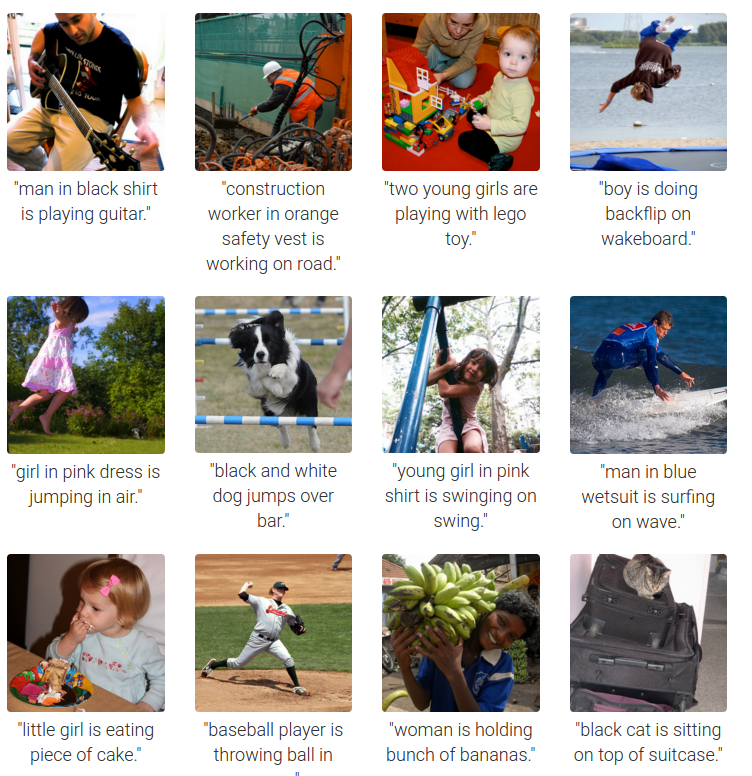
\includegraphics[scale=0.3]{img/deepVisual.png}
		\caption{Example results of the in \cite{Karpathy15} introduced model (source: http://cs.stanford.edu/people/karpathy/deepimagesent/}
		\label{fig:fig1.1}
	\end{center}
\end{figure}


A very promising area of image analysis are the so called \emph{neural networks}\footnote{See chapter 2.1.x}\nmc{NN}{Neural Networks}, which follow a machine learning approach. Their use, especially in the area of image classification and object recognition, made big breakthroughs possible in the recent past, e.g. Karpathy and Fei-Fei \cite{Karpathy15}, who created a neural network which is capable of describing an image or a scene with written text (see fig. 1.1 for some examples).

There is enormous potential in the use of neural networks in the digital pathology as well, but to transfer these algorithms and technologies, certain hindrances must be overcome. One of those hindrances is the need for proper training samples and an established ground truth\footnote{\emph{Ground truth} refers to a training sample whose outcome is known and validated as true.}. While generally there are huge amounts of whole slide images, most of them won't be usable without further preparation as a training sample. One way of preparing them are annotations. These can be added to the whole slide images, stored and later used for training.

Therefore the goal of this thesis is to give tools into the hands of pathologists to annotate whole slide images and save those annotations in such a way that they will be usable later in the combination with neural networks.


\section{Research Objective}
The objective of this thesis is the conceptualization and implementation of tools for whole slide images\footnote{See chapter 2.1.x}\nmc{WHI}{Whole Slide Image}, which allow for their annotation and a further usage in neural networks.
As a requirement, the tools have to be implemented in the form of microservices\footnote{See chapter 2.1.x}, each one with their own short documentation, including instructions for installation, usage and some examplary use cases. To achieve this goal, the implementation of 3 microservices is necessary.

The first microservice needs to be capable of converting a given set of image formats into the so called \emph{Deep Zoom Image Format}\footnote{See chapter 2.1.x}. The supported image formats are \emph{.bif, .mrxs, .ndpi, .scn, .svs, .svslide, .tif, .tiff, .vms} and \emph{.vmu}, in accordance with the capabilities of the Openslide framework\cite{Goode13}.

The second microservices task is to give a tool at hand with which a pathologist will be able to annotate all those whole slide images which were converted using the first microservice. Furthermore, the made annotations need to be persisted together with the highest resolution of the corresponding image.

The third microservice will be responsible for preparing the annotated whole slide images for the further usage in neural networks. For that purpose the service needs to be capable of dividing a single annotated whole slide image into multiple tiles, with the choice of either using the whole image or just the annotated areas. Furthermore, each tile needs enough information to reconstruct the whole image again afterwards.

\section{About this thesis}
Apart from the \emph{Introduction}, there are 5 more chapters in this thesis.

\emph{Chapter 2 - Background} defines some terminoligy and the general, required process chain which are all necessary to understand further chapters of this thesis. Furthermore, 3 microservices will be introduced in short.

\emph{Chapter 3 - Methodology} gives an overview over the current state of research for each microservice, as well as best practices. 

\emph{Chapter 4 - Implementation} goes into further details about how each microservice is implemented and which software and frameworks were used for that.

\emph{Chapter 5 - Discussion} will introduce a measurement for each microservice to measure its success. It will discuss the test setup as well as list the results.

\emph{Chapter 6 - Conclusion} will interpret the Results from Chapter 5 and analyze them closer. Furthermore, it will give an idea of what steps are to be taken next in the future.
\chapter{Background}
\section{Whole Slide Image Formats}
As the size of an acquired raw, uncompressed WSI is massive\footnote{ A typical 1,600 megapixel slide requires about 4.6 GB of memory on average\cite{Farahanil15}. The size of a H\&E (hematoxylin and eosin) stained slide ranges typically from 4 to 20 GB\cite{Singh11}.}, file formatting is required to mitigate the enormous amounts of information. Since there is no standardized format for WSIs, vendors came up with their own, proprietary solutions, which vary greatly\cite{Cornish13}. Efforts of standardization are being made through the \emph{Digital Imaging and Communications in Medicine} (DICOM) Standard\cite{DICOM10}\nmc{DICOM}{Digital Imaging and Communications in Medicine}.

Usually, WSI files are stored as a multitude of single images, spanning multiple folders and different resolutions. Those files are used to construct a so called \emph{image pyramid}\cite{Farahanil15} (see fig. 2.1 and the following DICOM Supplement 145 subsection).


\subsubsection{DICOM Supplement 145}
\cite{Singh11} describes DICOM as follows:
\begin{quotation}
	"Digital Imaging and Communications in Medicine (DICOM), synonymous with ISO (International Organization for Standardization) standard 12052, is the global standard for medical imaging and is used in all electronic medical record systems that include imaging as part of the patient record."
\end{quotation}

Before \emph{Supplement 145: Whole Slide Microscopic Image IOD and SOP Classes}, the DICOM Standard did not address standardization of WSI. Among others, the College of American Pathologist’s Diagnostic Intelligence and Health Information Technology Committee is responsible for the creation and further advancement of this supplement\cite{Singh11}.

It addresses every step involved in creating WSIs: image creation, acquisition, processing, analyzing, distribution, visualization and data management\cite{DICOM10}. It impacted the way how data is stored greatly\cite{Singh11}, due to the introduction of a pyramid image model\cite{DICOM10} (see fig. 2.1).

\begin{figure}[H]
	\begin{center}
		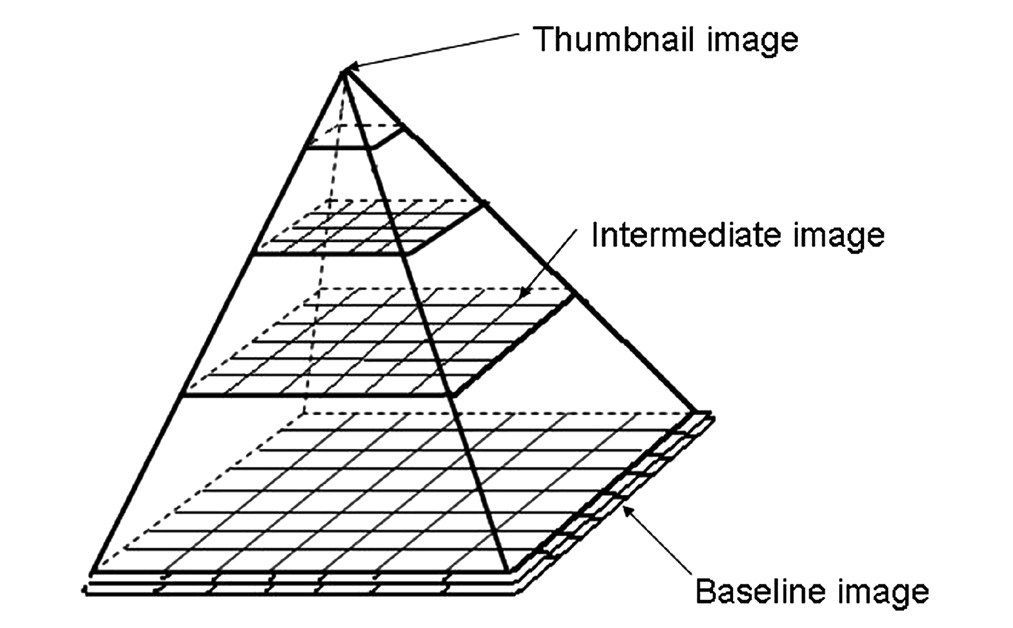
\includegraphics[scale=0.2]{img/imgPyramid.png}
		\caption{DICOMs image pyramid (source:\cite{Singh11})}
		\label{fig:fig2.1}
	\end{center}
\end{figure}

The image pyramid model facilitates rapid zooming and reduces the computational burden of randomly accessing and traversing a WSI\cite{Singh11},\cite{Park12}. This is made possible by storing an image in several precomputed resolutions, with the highest resolution sitting at the bottom (called the \emph{baseline image}) and a thumbnail or low power image at the top (compare fig. 2.1)\cite{DICOM10}. This creates a pyramid like stack of images, hence the name "pyramid model". The different resolutions are referred to as \emph{layers}\cite{DICOM10} or \emph{levels}\cite{Singh11} respectively.

Each level is tessellated into square or rectangular fragments, called tiles, and stored in a two dimensional array\cite{Farahanil15}. 

Because of this internal organization, the tiles of each level can be retrieved and put together separately, to either form a subregion of the image or show it entirely. This makes it easy to randomly access any subregion of the image without loading large amounts of data\cite{Singh11}.


\subsection{Proprietary Formats}
Vendors of whole slide scanners implement their own file formats, libraries and viewers (see tab. 2.1 for a list of vendors and their formats). Because of this, they can focus on the key features and abilities of their product. This generally leads to a higher usability, ease-of-use and enables highly tailored customer support. Furthermore, in comparison to open source projects, the longevity of proprietary software is often higher\cite{Optimus15}.

\begin{table}[H]
	\begin{center}
		\begin{tabular}{| l | l |}
			\hline
			\textbf{vendor} & \textbf{formats}\\ \hline
			Aperio & SVS, TIF\\ \hline
			Hamamatsu & VMS, VMU, NDPI\\ \hline
			Leica & SCN\\ \hline
			3DHistech/Mirax & MRXS\\ \hline
			Philips & TIFF\\ \hline
			Sakura & SVSLIDE\\ \hline
			Trestle & TIF\\ \hline
			Ventana & BIF, TIF\\ \hline
		\end{tabular}
		\caption{File formats by vendor}
	\end{center}
\end{table}

Since the proprietary formats have little to no documentation, most of the information presented here was reverse engineered in \cite{Goode13} and \cite{web:openslide}. All proprietary formats listed here implement a modified version of the pyramid model introduced in \cite{DICOM10}.


\subsubsection{Aperio}
The SVS format by Aperio is a TIFF-based format, which comes in a single file\cite{Goode13}. It has a specific internal organization in which the first image is the baseline image, which is always tiled (usually with 240x240 pixels). This is followed by a thumbnail, typically with dimensions of about 1024x768 pixels. The thumbnail is followed by at least one intermediate pyramid image (compare fig. 2.1), with the same compression and tile organization as the baseline image\cite{web:openslide}. Optionally, there may be a slide label and macro camera image at the end of each file\cite{web:openslide}.


\subsubsection{Hamamatsu}
Hamamatsu WSIs come in 3 variants:
\begin{enumerate}[(1)]
	\item VMS
	\item VMU
	\item NDPI
\end{enumerate}

(1) and (2) consist of an index file ((1) - [file name].vms, (2) - [file name].vmu) and 2 or more image files. In the case of (2), there is also an additional optimization file. (3) consists of a single TIFF-like file with custom TIFF tags. While (1) and (3) contain jpeg images, (2) contains a custom, uncompressed image format called \emph{NGR}\footnote{For more information on NGR, consult \url{http://openslide.org/formats/hamamatsu/}}\cite{web:openslide}.

The random access support for decoding parts of jpeg files is poor. To get around this, so called \emph{restart markers}\footnote{Restart markers were originally designed for error recovery. The markers allow the decoder to resynchronize at set intervals throughout the image\cite{Goode13}.} are used to create virtual slides\cite{Goode13}. The markers are placed at regular intervals. The offset of every marker is specified in different manner. In the case of (1), it can be found in the index file. In the case of (2), the optimization file holds the information and in the case of (3), a TIFF tag contains the offset\cite{web:openslide}.


\subsubsection{Leica}
SCN is a single file format based on BigTIFF, additionally .scn provides a pyramidal thumbnail image.\cite{Goode13}.

The first TIFF directory has a tag called "ImageDescription" which contains an XML document that defines the internal structure of the WSI\cite{web:openslide}.

Leica WSIs are structured as a collection of images, each of which has multiple pyramid levels. While the collection only has a size, images have a size and position, all measured in nanometers. Each dimension has a size in pixels, an optional focal plane number, and a TIFF directory containing the image data. Fluorescence images have different dimensions (and thus different TIFF directories) for each channel\cite{web:openslide}.

Brightfield slides have at least two images: a low-resolution macro image and one or more main images corresponding to regions of the macro image. Fluorescence slides can have two macro images: one brightfield and one fluorescence\cite{web:openslide}.


\subsubsection{3DHistech/Mirax}
MRXS is a multi-file format with very complicated metadata in a mixture of text and binary formats. Images are stored as either JPEG, PNG or BMP\cite{Goode13}. The poor handling of random access is also applicable to PNG. Because of this, multiple images are needed to encode a single slide image. To avoid having many individual files, images are packed into a small number of data files. An index file provides offsets into the data files for each required piece of data.\cite{web:openslide}. 

A 3DHistech/Mirax scanner take images with an overlap. Each picture taken is then tessellated without an overlap. Therefore, they only occur between taken pictures\cite{web:openslide}.

The generation of the image pyramid differs from the process described in 2.1. To create the $n^{th}$ level, each image of the $n^{th}-1$ level is divided by 2 in each dimension and then concatenated into a new image. Where the $n^{th}-1$ level had 4 images in 2x2 neighborhood, the $n^{th}$ level will only have 1 image. This process has no regards for overlaps. Thus, overlaps may occur in the higher levels of the image pyramid\cite{web:openslide}.


\subsubsection{Philips}
Philips' TIFF is an export from the native iSyntax format. An XML document with the hierarchical structure of the WSI can be found over the \emph{ImageDescription} tag of the first TIFF directory. It contains key-value pairs based on DICOM tags\cite{web:openslide}.

Slides with multiple regions of interest are structured as a single image pyramid enclosing all regions. Slides may omit pixel data for TIFF tiles not in an ROI. When such tiles are downsampled into a tile that does contain pixel data, their contents are rendered as white pixels\cite{web:openslide}.

Label and macro images are stored either as JPEG or as stripped TIFF directories.


\subsubsection{Sakura}
WSIs in the SVSLIDE format are SQLite 3 database files. Their tables contain the metadata, associated images and tiles in the JPEG format. The tiles are addressed as (focal plane, downsample, level-0 X coordinate, level-0 Y coordinate, color channel). Additionally, each color channel has a separate grayscale image\cite{web:openslide}.


\subsubsection{Trestle}
Trestles TIF is a single-file TIFF. The WSI has the standard pyramdic scheme and tessellation. It contains non-standard metadata and overlaps, which are specified in additional files. The first image in the TIFF file is the baseline image. Subsequent images are assumed to be consecutive levels of the image pyramid with decreasing resolution\cite{web:openslide}.


\subsubsection{Ventana}
Ventanas WSIs are single-file BigTIFF images, organized in the typical pyramidical scheme. The images are tiled and have non-standard metadata, as well as overlaps. They come with a macro and a thumbnail image\cite{web:openslide}.

	
\subsection{Open Formats}
As mentioned in 2.1.1, proprietary formats typically come without much or any documentation. Furthermore, a vendors viewer is usually the only way of viewing WSIs of a particular format. This creates a vendor lock-in, where users can't take advantage of new improvements offered by other vendors. Furthermore, most viewers only provide support for Windows platforms. While, in a clinical setting, Windows may dominate the market, a significant amount of users in medical research prefer Linux or Mac OS X\cite{Goode13}. The use of mobile platforms, such as iOS or Android tablets may also have a great influence of the work flow in the future. Some vendors try to compensate for this fact with a server-based approach, which hurts performance by adding a network round-trip delay on every digital slide operation\cite{Goode13}.

To compensate those issues, open image formats have been suggested, which will be discussed further, in the following subsections.


\subsubsection{Deep Zoom Images}
The Deep Zoom Image (DZI)\nomenclature{DZI}{Deep Zoom Image} format is an XML-based file format, developed and maintained by Microsoft\cite{web:dzi}. A DZI is a pyramidcal, tiled image (see fig. 2.2), similar to the one described in \cite{DICOM10} (compare fig 2.1 and 2.2), with two exceptions:
\begin{enumerate}
	\item the baseline image is referred to as the highest level, instead of the lowest; this either turns the image pyramid or its labeling upside down
	\item tiles are always square, with the exception of the last column/row
\end{enumerate}

\begin{figure}[H]
	\begin{center}
		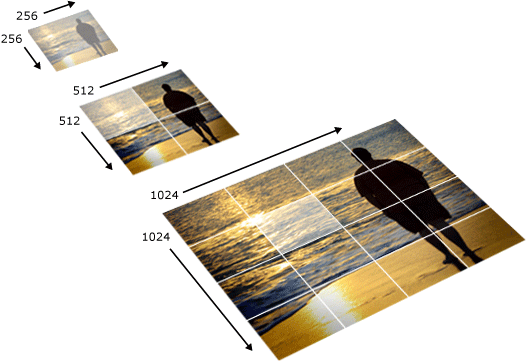
\includegraphics[scale=0.4]{img/dzi_pyramid.png}
		\caption{DZI pyramid model example (source:\cite{web:dzi})}
		\label{fig:fig2.2}
	\end{center}
\end{figure}

A DZI consists of two main parts\cite{web:dzi}: 
\begin{enumerate}[(1)]
	\item a describing XML file ([file name].dzi) with informations about:
	\begin{itemize}
		\item the format of single tiles (e.g. JPEG or PNG)
		\item overlap between tiles
		\item size of tiles
		\item height and width of baseline image
	\end{itemize}
	\item a directory ([file name]{\textunderscore}files) with image tiles of the specified format
\end{enumerate}

(1) and (2) are stored "next" to each other, so that there are 2 spearate files. (2) contains sub directories, one for each level of the image pyramid. The baseline image of a DZI is in the highest level. Each level is tessellated into as many tiles necessary to go over the whole image, with each tile having the size specified in the XML file. If the image size is no multiple of the specified tile size, the width of the $n^{th}$ column of tiles will be $(width \mod tile$ $size)$ pixels. Equally, the height of the $m^{th}$ row will be $(height \mod tile$ $size)$ pixels. Thus, the outermost right bottom tile $t_{n,m}$ will be of $(width \mod tile$ $size)$ x $(height \mod tile$ $size)$ pixels.


\subsubsection{International Image Interoperability Framework}
The International Image Interoperability Framework (IIIF)\nmc{IIIF}{International Image Interoperability Framework} is the result of a cooperation between The British Library, Stanford University, the Bodleian Libraries\footnote{Oxford University}, the Bibliothèque Nationale de France, Nasjonalbiblioteket\footnote{National Library of Norway}], Los Alamos National Laboratory Research Library and Cornell University\cite{Cramer11}. Version 1.0 was published in 2012.

IIIFs goal is to collaboratively produce an interoperable technology and community framework for image delivery\cite{web:iiif2}. To achieve this, IIIF tries to:
\begin{enumerate}[(1)]
	\item give scholars access to image-based resources around the world
	\item define a set of common APIs to support interoperability between image repositories
	\item develop and document shared technologies (such as image servers and web clients), that enable scholars to view, compare, manipulate and annotate images
\end{enumerate}

\begin{figure}[H]
	\begin{center}
		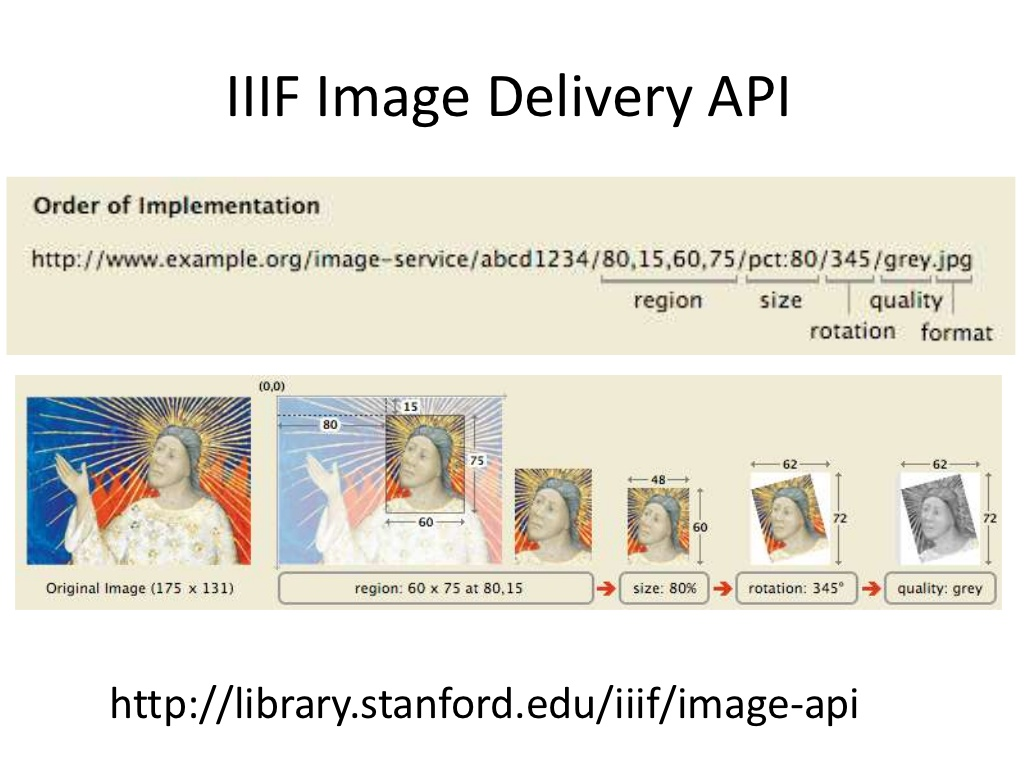
\includegraphics[scale=0.3]{img/iiif_url_example.jpg}
		\caption{Example of iiif request (source:\url{http://www.slideshare.net/Tom-Cramer/iiif-international-image-interoperability-framework-dlf2012?ref=https://www.diglib.org/forums/2012forum/transcending-silos-leveraging-linked-data-and-open-image-apis-for-collaborative-access-to-digital-facsimiles/})}
		\label{fig:fig2.3}
	\end{center}
\end{figure}

The relevant part for this thesis is (2), especially the image API\cite{web:iiif}. It specifies a web service that returns an image in response to a standard web request. The URL can specify the region, size, rotation, quality and format of the requested image (see fig. 2.3). Originally intended for resources in digital image repositories maintained by cultural heritage organizations, the API can be used to retrieve static images in response to a properly constructed URL\cite{web:openseadragon}. The URL scheme looks like this\cite{web:iiif}:
\begin{lstlisting}
{scheme}://{server}{/prefix}/{identifier}/{region}/{size}/{rotation}/{quality}.{format}
\end{lstlisting}

The \emph{region} and \emph{size} parameters are of special interest for this thesis\footnote{For detailed information on all parameters see the official API: \url{http://iiif.io/api/image/2.0}}. With them, it is possible to request only a certain region of an image in a specified size.

The region parameter defines the rectangular portion of the full image to be returned. It can be specified by pixel coordinates, percentage or by the value “full” (see tab. 2.2 and fig. 2.4).

\begin{table}[H]
	\begin{center}
		\begin{tabular}{| p{2cm} | p{9cm} |}
			\hline
			\textbf{Form} & \textbf{Description}\\ \hline
			full & The complete image is returned, without any cropping.\\ \hline
			x,y,w,h & The region of the full image to be returned is defined in terms of absolute pixel values. The value of x represents the number of pixels from the 0 position on the horizontal axis. The value of y represents the number of pixels from the 0 position on the vertical axis. Thus the x,y position 0,0 is the upper left-most pixel of the image. w represents the width of the region and h represents the height of the region in pixels.\\ \hline
			pct:x,y,w,h & The region to be returned is specified as a sequence of percentages of the full image’s dimensions, as reported in the Image Information document. Thus, x represents the number of pixels from the 0 position on the horizontal axis, calculated as a percentage of the reported width. w represents the width of the region, also calculated as a percentage of the reported width. The same applies to y and h respectively. These may be floating point numbers.\\ \hline
		\end{tabular}
		\caption{Valid values for \emph{region} parameter (source:\cite{web:iiif})}
	\end{center}
\end{table}

If the request specifies a regions whose size extends beyond the actual size of the image, the response should be a cropped image, instead of an image with added empty space. If the region is completely outside of the image, the response should be a 404 http status code\cite{web:iiif}.

\begin{figure}[H]
	\begin{center}
		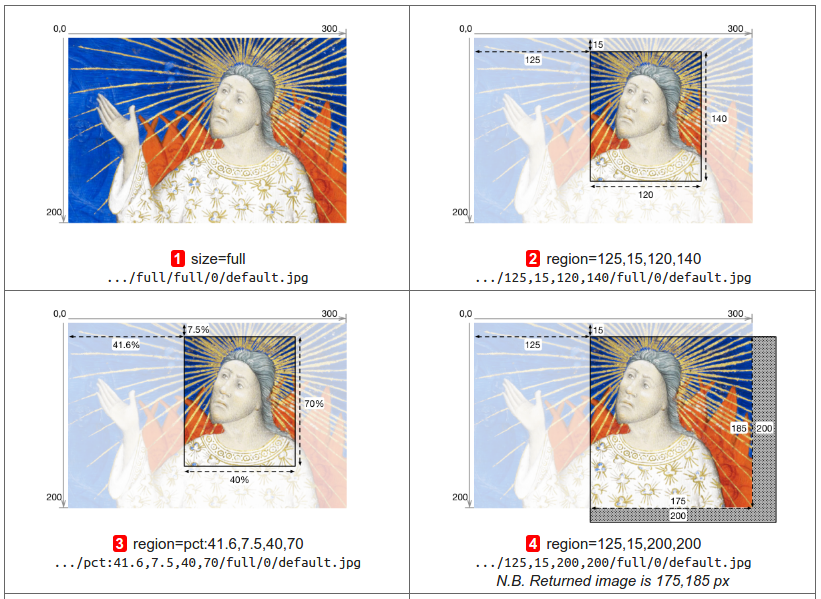
\includegraphics[scale=0.4]{img/region_param.png}
		\caption{Results of IIIF request with different values for region parameter (source:\cite{web:iiif})}
		\label{fig:fig2.4}
	\end{center}
\end{figure}

If a region was extracted, it is scaled to the dimensions specified by the size parameter (see tab. 2.3 and fig. 2.5).

\begin{figure}[H]
	\begin{center}
		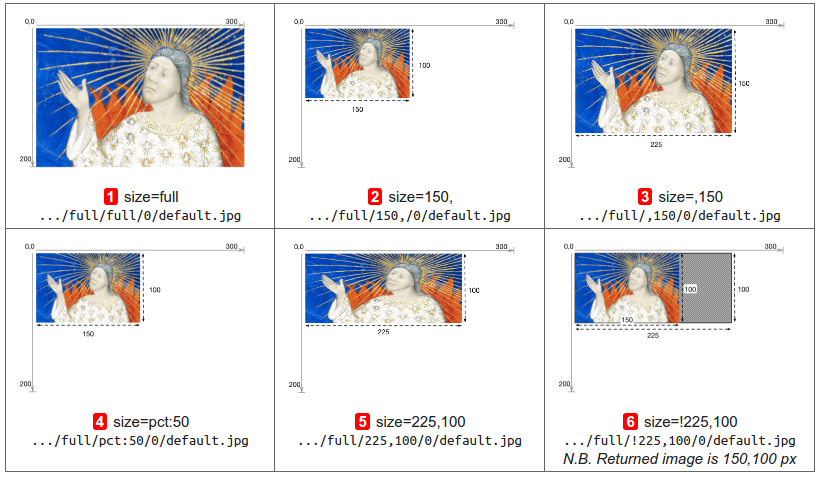
\includegraphics[scale=0.35]{img/size_parameter.png}
		\caption{Results of IIIF request with different values for size parameter (source:\cite{web:iiif})}
		\label{fig:fig2.5}
	\end{center}
\end{figure}

If the resulting height or width equals 0, then the server should return a 400 http status code. Depending on the image server, scaling above the full size of the extracted region may be supported\cite{web:iiif}.

\begin{table}[H]
	\begin{center}
		\begin{tabular}{| p{2cm} | p{9cm} |}
			\hline
			\textbf{Form} & \textbf{Description}\\ \hline
			full & The extracted region is not scaled, and is returned at its full size.\\ \hline
			w, & The extracted region should be scaled so that its width is exactly equal to w, and the height will be a calculated value that maintains the aspect ratio of the extracted region.\\ \hline
			,h & The extracted region should be scaled so that its height is exactly equal to h, and the width will be a calculated value that maintains the aspect ratio of the extracted region.\\ \hline
			pct:n & The width and height of the returned image is scaled to n\% of the width and height of the extracted region. The aspect ratio of the returned image is the same as that of the extracted region.\\ \hline
			w,h & The width and height of the returned image are exactly w and h. The aspect ratio of the returned image may be different than the extracted region, resulting in a distorted image.\\ \hline
			!w,h & The image content is scaled for the best fit such that the resulting width and height are less than or equal to the requested width and height. The exact scaling may be determined by the service provider, based on characteristics including image quality and system performance. The dimensions of the returned image content are calculated to maintain the aspect ratio of the extracted region.\\ \hline
		\end{tabular}
		\caption{Valid values for \emph{size} parameter (source:\cite{web:iiif})}
	\end{center}
\end{table}

To use the IIIF API, a compliant web server must be deployed. There are 2 alternatives to set up a new one\cite{web:openseadragon},\cite{web:iiif2}:
\begin{itemize}
	\item \textbf{Loris}, an open source image server based on python that supports the IIIF API versions 2.0, 1.1 and 1.0. Supported image formats are JPEG, JPEG2000 and TIFF.
	\item \textbf{IIPImage Server}, an open source Fast CGI module written in C++, that is designed to be embedded within a hosting web server such as Apache, Lighttpd, MyServer or Nginx. Supported image formats are JPEG2000 and TIFF.
\end{itemize}


\subsubsection{JPEG2000}
\subsubsection{Open Street Maps}
\subsubsection{TIFF/BigTIFF}
\subsubsection{Tiled Map Service}


\subsection{Choice of Format}


\section{Short Introduction to Neural Networks}
The objective of this thesis ultimately is to create training samples for NN\footnote{compare chap. 1.2}. Before going into other details, it is necessary to clarify what NN are, how they work, why they need training samples and what they use them for\footnote{It should be mentioned that the scope of NN is huge and worth a whole thesis by themselves. This is nothing more than a short introduction and further consultation of literature (e.g. \cite{Stergiou96},\cite{Bourg04},\cite{Egmont-Petersen02},\cite{Kriesel07},\cite{Shiffman12}) is highly recommended.}.

Artificial Neural Networks (NN)\nmc{NN}{Neural Networks} are a group of models inspired by Biological Neural Networks (BNN) \nmc{BNN}{Biological Neural Networks}. BNNs can be described as an interconnected web of neurons (see fig 2.x), whose purpose it is to transmit information in the form of electrical signals. A neuron receives input via dendrites and send output via axons\cite{Shiffman12}. An average human adult brain contains about $10^{11}$ neurons. Each of those receives input from about $10^4$ other neurons. If their combined input is strong enough, the receiving neuron will send an output signal to other neurons\cite{Bourg04}.

\begin{figure}[H]
	\begin{center}
		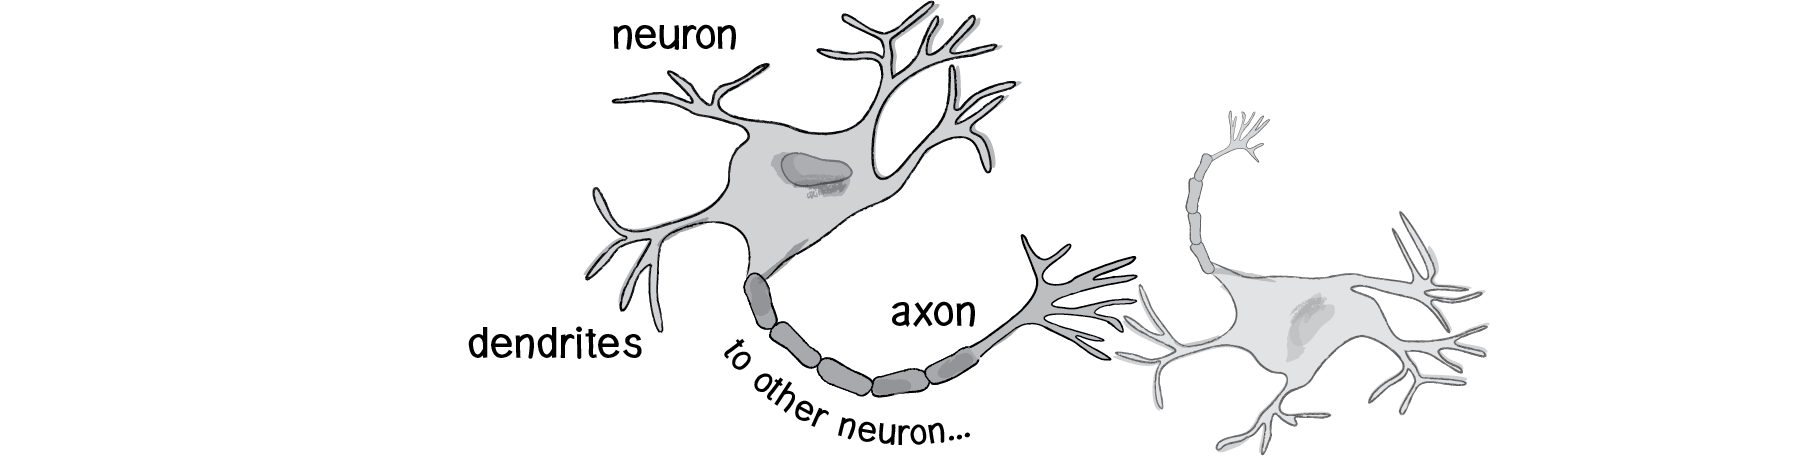
\includegraphics[scale=0.7]{img/bnn.png}
		\caption{Neuron in a BNN (source:\cite{Shiffman12})}
		\label{fig:fig2.2}
	\end{center}
\end{figure}

NN are much simpler in comparison\footnote{Usually, they don't have much more than a few dozen neurons\cite{Bourg04}.}, but generally work in the same fashion.

One of the biggest strengths of a NN, much like a BNN, is the ability to adapt by learning\footnote{As humans, NN learn by training\cite{Shiffman12}.}. This adaption is based on \emph{weights} that are assigned to the connections between single neurons. Fig 2.x shows an exemplary NN with neurons and the connections between them.

\begin{figure}[H]
	\begin{center}
		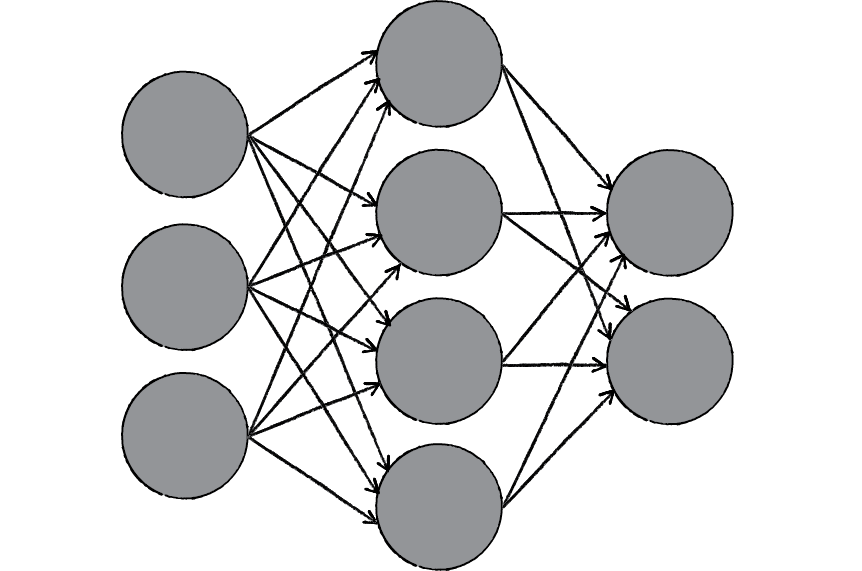
\includegraphics[scale=1.0]{img/NN.png}
		\caption{Exemplary NN (source:\cite{Shiffman12})}
		\label{fig:fig2.3}
	\end{center}
\end{figure}

Each line in fig, 2.x represents a connection between 2 neurons. Those connections are a one-directional flow of information, each assigned with a specific weight. This weight is a simple number that is multiplied with the incoming/outgoing signal and therefore weakens or enhances it. They are the defining factor of the behavior of a NN. Determining those values is the purpose of training a NN\cite{Bourg04}.

According to \cite{Shiffman12}, some of the standard use cases for NN are:

\begin{itemize}
	\item Pattern Recognition
	\item Time Series Prediction
	\item Signal Processing Perceptron
	\item Control
	\item Soft Sensors
	\item Anomaly Detection
\end{itemize}


\subsection{Methods of Learning}
There are 3 general strategies when it comes to the training of a NN\cite{Bourg04}. Those are:

\begin{enumerate}
	\item Supervised Learning
	\item Unsupervised Learning
	\item Reinforcement Learning (a variant of Unsupervised Learning\cite{Rojas96})
\end{enumerate}

\emph{Supervised Learning} is a strategy that involves a training set to which the correct output is known, as well as an observing teacher. The NN is provided with the training data and computes its output. This output is compared to the expected output and the difference is measured. According to the error made, the weights of the NN are corrected. The magnitude of the correction is determined by the used learning algorithm\cite{Rojas96}.

\emph{Unsupervised Learning} is a strategy that is required when the correct output is unknown and no teacher is available. Because of this, he NN must organize itself\cite{Shiffman12}. \cite{Rojas96} makes a distinction between 2 different classes of unsupervised learning:

\begin{itemize}
	\item reinforced learning
	\item competitive learning
\end{itemize}

Reinforced learning adjusts the weights in such a way, that desired output is reproduced. For example, a robot in a maze. If the robot can drive straight without any hindrances, it can associate this sensory input with driving straight (desired outcome). As soon as it approaches a turn, the robot will hit a wall (non-desired outcome). To prevent it from hitting the wall it must turn, therefore the weights of turning must be adjusted to the sensory input of being at a turn. Another example is \emph{Hebbian learning}\footnote{see \cite{Rojas96} for further information}\cite{Rojas96}.

In competitive learning, the single neurons compete against each other for the right to give a certain output for an associated input. Only one element in the NN is allowed to answer, so that other, competing neurons are inhibited\cite{Rojas96}.


\subsection{The Perceptron}
The perceptron was invented by Rosenblatt at the Cornell Aeronautical Laboratory in 1957\cite{Rosenblatt58}. It is the computational model of a single neuron and as such, the simplest NN possible\cite{Shiffman12}. A perceptron consists of one or more inputs, a processor and a single output (see fig. 2.x)\cite{Rosenblatt58}.

\begin{figure}[H]
	\begin{center}
		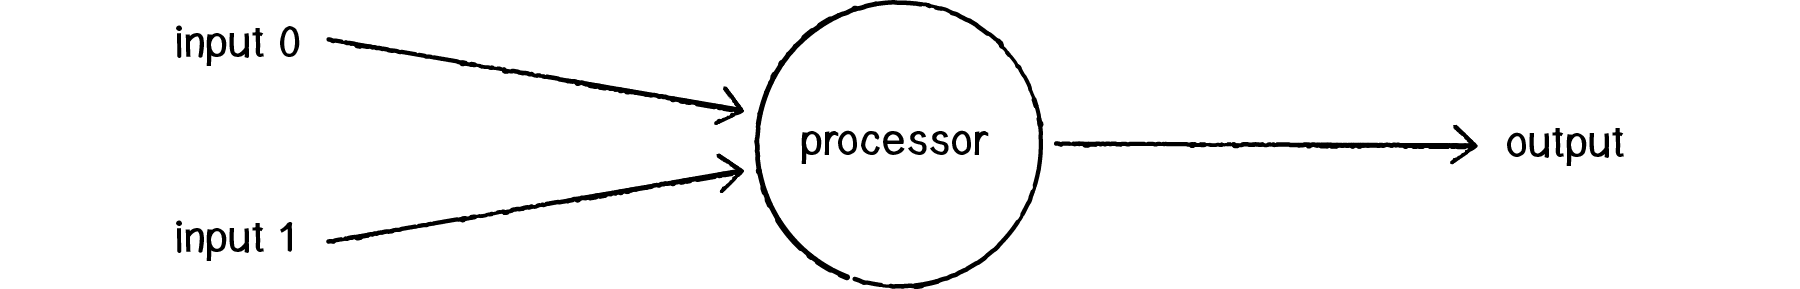
\includegraphics[scale=0.7]{img/perceptron.png}
		\caption{Perceptron by Rosenblatt (source:\cite{Shiffman12})}
		\label{fig:fig2.5}
	\end{center}
\end{figure}

This can be directly compared to the neuron in fig. 2.x, where:
\begin{itemize}
	\item input = dendrites
	\item processor = cell
	\item output = axon
\end{itemize}

A perceptron is only capable of solving \emph{linearly separable} problems, such as logical \emph{AND} and \emph{OR} problems. To solve non-linearly separable problems, more then one perceptron is required\cite{Rosenblatt58}. Simply put, a problem is linearly separable, if it can be solved with a straight line (see fig. 2.x), otherwise it is considered a non-linearly separable problem (see fig. 2.x).

\begin{figure}[H]
	\begin{center}
		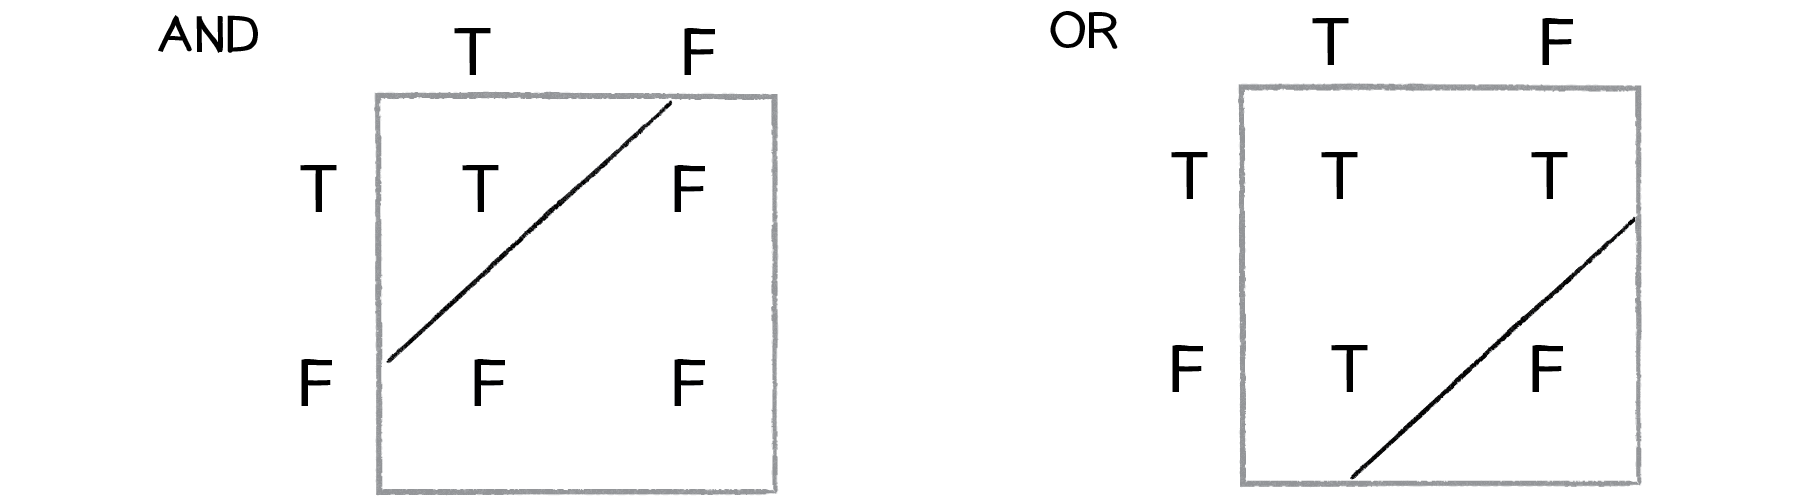
\includegraphics[scale=0.6]{img/lsp.png}
		\caption{Examples for linearly separable problems (source:\cite{Shiffman12})}
		\label{fig:fig2.7}
	\end{center}
\end{figure}

\begin{figure}[H]
	\begin{center}
		
\includegraphics[scale=0.75]{img/nlsp.png}
		\caption{Examples for non-linearly separable problems (source:\cite{Shiffman12})}
		\label{fig:fig2.8}
	\end{center}
\end{figure}


\subsection{Multi-layered Neural Networks}
To solve more complex problems, multiple perceptrons can be connected to from a more powerful NN. A single perceptron might not be able to solve \emph{XOR}, but one perceptron can solve \emph{OR}, while the other can solve \emph{$\neg$AND}. Those two perceptrons combined can solve \emph{XOR}\cite{Shiffman12}.

If multiple perceptrons get combined, they create layers. Those layers can be separated into 3 distinct types\cite{Stergiou96}:
\begin{itemize}
	\item input layer
	\item hidden layer
	\item output layer
\end{itemize}

A typical NN will have an input layer, which is connected to a number of hidden layers, which either connect to more hidden layers or, eventually, an output layer (see fig. 2.x for a NN with one hidden layer).

\begin{figure}[H]
	\begin{center}
		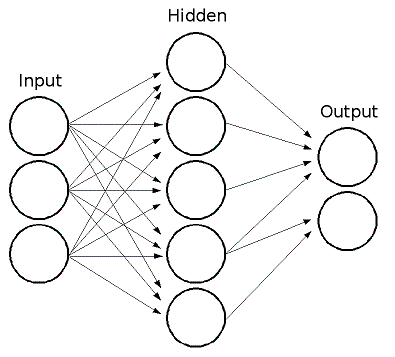
\includegraphics[scale=0.8]{img/mlp.png}
		\caption{NN with multiple layers (source: \url{http://docs.opencv.org/2.4/_images/mlp.png)}}
		\label{fig:fig2.2}
	\end{center}
\end{figure}

As the name suggests, the input layer gets provided with the raw information input. Depending on the internal weights and connections inside the hidden layer, a representation of the input information gets formed. At last, the output layer generates output, again based on the connections and weights of the hidden and output layer\cite{Stergiou96}.

Training this kind of NN is much more complicated than training a simple perceptron, since weights are scattered all over the NN and its layers. A solution to this problem is called \emph{backpropagation}\cite{Shiffman12}.


\subsubsection{Backpropagation}
Training is an optimization process. To optimize something, a metric to measure has to be established. In the case of backpropagation, this metric is the accumulated output error of the NN to a given input\footnote{To do so, it is necessary to know the right answer. Therefore, backpropagation is part of the supervised learning process.}. There are several ways to calculate this error, with the \emph{mean square error}\footnote{Mean square error is the average of the square of the differences of two variables, in this case the expected and the actual output.} being the most common one\cite{Bourg04}.

Finding the optimal weights is an iterative process of the following steps:
\begin{enumerate}
	\item start with training set of data with known output
	\item initialize weights in NN
	\item for each set of input, feed the NN and compute the output
	\item compare calculated with known output
	\item adjust weights to reduce error
\end{enumerate}

There are 2 possibilities in how to proceed. The first one is to compare results and adjust weights after each input/output-cycle. The second one is to calculate the accumulated error over a whole iteration of the input/output-cycle. Each of those iterations is known as an \emph{epoch}\cite{Bourg04}.


\section{Microservices}
The following section elaborates on the concept of \emph{Microservices} (MS)\nmc{MS}{Microservice}, defining what they are, listing their pros and cons, as well as explaining why this approach was chosen over a monolithic approach. A monolithic software solution is described by \cite{Lewis14} as follows:
\begin{quotation}
	"[...] a monolithic application [is] built as a single unit. Enterprise Applications are often built in three main parts: a client-side user interface (consisting of HTML pages and javascript running in a browser on the user's machine) a database (consisting of many tables inserted into a common, and usually relational, database management system), and a server-side application. The server-side application will handle HTTP requests, execute domain logic, retrieve and update data from the database, and select and populate HTML views to be sent to the browser. This server-side application is a monolith - a single logical executable. Any changes to the system involve building and deploying a new version of the server-side application."
\end{quotation}


\subsection{Definition}
MS are an interpretation of the Service Oriented Architecture. The concept is to separate one monolithic software construct into several smaller, modular pieces of software\cite{Wolff16}. As such, MS are a modularization concept. However, they differ from other such concepts, since MS are independent from each other. This is a trait, other modularization concepts usually lack\cite{Wolff16}. As a result, changes in one MS don't bring up the necessity of deploying the whole product cycle again, but just the one service. This can be achieved by turning each MS into an independent process with its own runtime\cite{Lewis14}.

This modularization creates an information barrier between different MS. Therefore, if MS need to share data or communicate with each other, light weight communication mechanisms must be established, such as a RESTful API\cite{Riggins15}.

Even though MS are more a concept than a specific architectural style, certain traits are usually shared between them\cite{Riggins15}. According to \cite{Riggins15} and \cite{Lewis14}, those are:

\begin{enumerate}[(a)]
	\item \textbf{Componentization as a Service:} bringing chosen components (e.g. external libraries) together to make a customized service
	\item \textbf{Organized Around Business Capabilities:} cross-functional teams, including the full range of skills required to achieve the MS goal
	\item \textbf{Products instead of Projects:} teams own a product over its full lifetime, not just for the remainder of a project
	\item \textbf{Smart Endpoints and Dumb Pipes:} each microservice is as decoupled as possible with its own domain logic
	\item \textbf{Decentralized Governance:} enabling developer choice to build on preferred languages for each component.
	\item \textbf{Decentralized Data Management:} having each microservice label and handle data differently
	\item \textbf{Infrastructure Automation:} including automated deployment up the pipeline
	\item \textbf{Design for Failure:} a consequence of using services as components, is that applications need to be designed so that they can tolerate the failure of single or multiple services
\end{enumerate}

Furthermore, \cite{Bugwadia15} defined 5 architectural constraints, which should help to develop a MS:

\begin{enumerate}[(1.)]
	\item \textbf{Elastic}\\
	The elasticity constraint describes the ability of a MS to scale up or down, without affecting the rest of the system. This can be realized in different ways. \cite{Bugwadia15} suggests to architect the system in such a fashion, that multiple stateless instances of each microservice can run, together with a mechanism for Service naming, registration, and discovery along with routing and load-balancing of requests.
	\item \textbf{Resilient}\\
	This constraint is referring to the before mentioned trait (h) - \emph{Design for Failure}. The failure of or an error in the execution of a MS must not impact other services in the system.
	\item \textbf{Composable}\\
	To avoid confusion, different MS in a system should have the same way of identifying, representing, and manipulating resources, describing the API schema and supported API operations.
	\item \textbf{Minimal}\\
	A MS should only perform one single business function, in which only semantically closely related components are needed.
	\item \textbf{Complete}\\
	A MS must offer a complete functionality, with minimal dependencies to other services. Without this constraint, services would be interconnected again, making it impossible to upgrade or scale individual services.
\end{enumerate}


\subsection{Advantages and Disadvantages}
% pros
One big advantage of this modularization is that each service can be written in a different programming language, using different frameworks and tools. Furthermore, each microservice can bring along its own support services and data storages. It is imperative for the concept of modularization, that each microservice has its own storage of which it is in charge of\cite{Wolff16}.

The small and focused nature of MS makes scaling, updates, general changes and the deploying process easier. Furthermore, smaller teams can work on smaller code bases, making the distribution of know how easier\cite{Riggins15}.

Another advantage is how well MS plays into the hands of agile, scrum and continuous software development processes, due to their previously discussed inherent traits.

% cons
The modularization of MS doesn't only yield advantages. Since each MS has its own, closed off data management\footnote{See 2.3.1(f) (\emph{Decentralized Data Management})}, interprocess communication becomes a necessity. This can lead to communicational overhead which has a negative impact on the overall performance of the system\cite{Wolff16}.

2.3.1(e) (\emph{Decentralized Governance}) can lead to compatibility issues, if different developer teams chose to use different technologies. Thus, more communication and social compatibility between teams is required. This can lead to an unstable system which makes the deployment of extensive workarounds necessary\cite{Riggins15}.

It often makes sense to share code inside a system to not replicate functionality which is already there and therefore increase the maintenance burden. The independent nature of MS can make that very difficult, since shared libraries must be build carefully and with the fact in mind, that different MS may use different technologies, possibly creating dependency conflicts.


\subsection{Conclusion}	
After consideration of the advantages and disadvantages of MS, the author decided in favor of using them. This is mainly due to the fact of working alone on the project, negating some of their inherent disadvantages:
\begin{itemize}
	\item Interprocess communication doesn't arise between the single stages of the process chain, since they have a set order\footnote{E.g. it wouldn't make sense trying extract a training sample without converting or annotating a WSI first.}
	\item Different technologies may be chosen for the single steps of the process chain, however, working alone on the project makes technological incompatibilities instantly visible
	\item The services shouldn't share functionality, therefore there should be no need for shared libraries
\end{itemize}
This makes the advantages outweight the disadvantages clearly:
\begin{itemize}
	\item different languages and technologies can be used for every single step of the process chain, making the choice of the most fitting tool possible
	\item WSIs take a heavy toll on memory and disk space due to their size; the use of MS allows each step of the chain to handle those issues in the most suitable way for each given step
	\item separating the steps of the process chain into multiple MS makes for a smaller and easier maintainable code base
	\item other bachelor/master students may continue to use or work on this project in the future, making the benefit of a small, easily maintainable code base twice as important
	\item the implementation of the project will happen in an iterative, continuous manner, which is easily doable with the use of MS
\end{itemize}


\section{Process Chain}
This section and its following subsections are dedicated to establish the process chain necessary to accomplish the research objectives stated in 1.2(a) - 1.2(c). The usual procedure would look as follows:

\begin{enumerate}[(1.)]
	\item convert chosen WSI $img^{wsi}_i$ to DZI format $img^{dzi}_i$
	\item open $img^{dzi}_i$ in a viewer $V$
	\item annotate $img^{dzi}_i$ in $V$
	\item persist annotations $A_i$ on $img^{dzi}_i$ in a file $f_{(A_i)}$
	\item create training sample $ts_i$ by extracting the information of $A_i$ in correspondence to $img^{dzi}_i$
\end{enumerate}

While it only makes sense to run (1.) once per $img^{wsi}_i$ to create $img^{dzi}_i$, steps (2.) - (4.) can be repeated multiple times, so that there is no need to finish the annotation of an image in one session. That makes it necessary to not only save but also load annotations. Therefore, the loading of already made annotations can be added as step (2.5). This also enables the user of editing and deleting already made annotations. Because of this, step (5.) also needs to be repeatable.

The single steps of the process chain will be sorted into semantic groups. Each group will be realized by its own MS, as stated in 2.3. The semantic groups are: conversion (1.), extraction (5.) and viewing and annotation (2. - 4.).

A MS will be introduced for each group in the following subsections(2.4.1 - 2.4.3). Those are:

\begin{itemize}
	\item \textbf{Conversion Service}\\
	This service will be responsible of the conversion from $img^{wsi}_i$ to $img^{dzi}_i$ (1.).
	\item \textbf{Annotation Service}\\
	This service will offer a GUI to view a $img^{dzi}_i$, as well as make and manage annotations (2. - 4.)
	\item \textbf{Tessellation Service}\\
	This service will be responsible for extracting a $ts_i$ from a given $A_i$ and $img^{dzi}_i$ (5.).
\end{itemize}


\subsection{Conversion Service}

The devices which create WSIs, so called \emph{whole slide scanners}, create images in various formats, depending on the producer and a lack of a defined standard\cite{Cornish13}. The Conversion Service (CS)\nmc{CS}{Conversion Service} has the goal of converting those formats to DZI\footnote{see chap. 1.2(i) and 1.2(ii) for the reasons}].

\begin{figure}[H]
	\begin{center}
		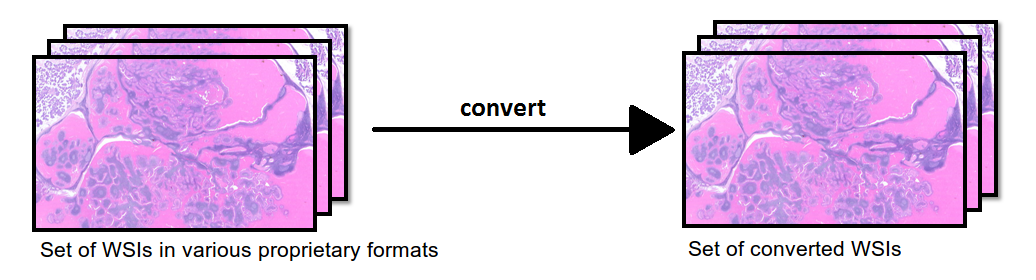
\includegraphics[scale=0.35]{img/processChainA.png}
		\caption{Visualization of the Conversion Service}
		\label{fig:fig2.1}
	\end{center}
\end{figure}

Upon invocation, the CS will take every single WSI inside a given directory and convert it to DZI. The output of each conversion will be saved in another specified folder. Valid image formats for conversion are:

\begin{itemize}
	\item .bif
	\item .mrxs
	\item .ndpi
	\item .scn
	\item .svs
	\item .svslide
	\item .tif
	\item .tiff
	\item .vms
	\item .vmu
\end{itemize}


\subsection{Annotation Service}
As mentioned in 2.4, the Annotation Service (AS)\nmc{AS}{Annotation Service} will provide a graphical user interface (GUI)\nmc{GUI}{Graphical User Interface} to view a DZI, make annotations and manage those annotations. This also includes persisting made annotations in a file (see fig. 2.2).

\begin{figure}[H]
	\begin{center}
		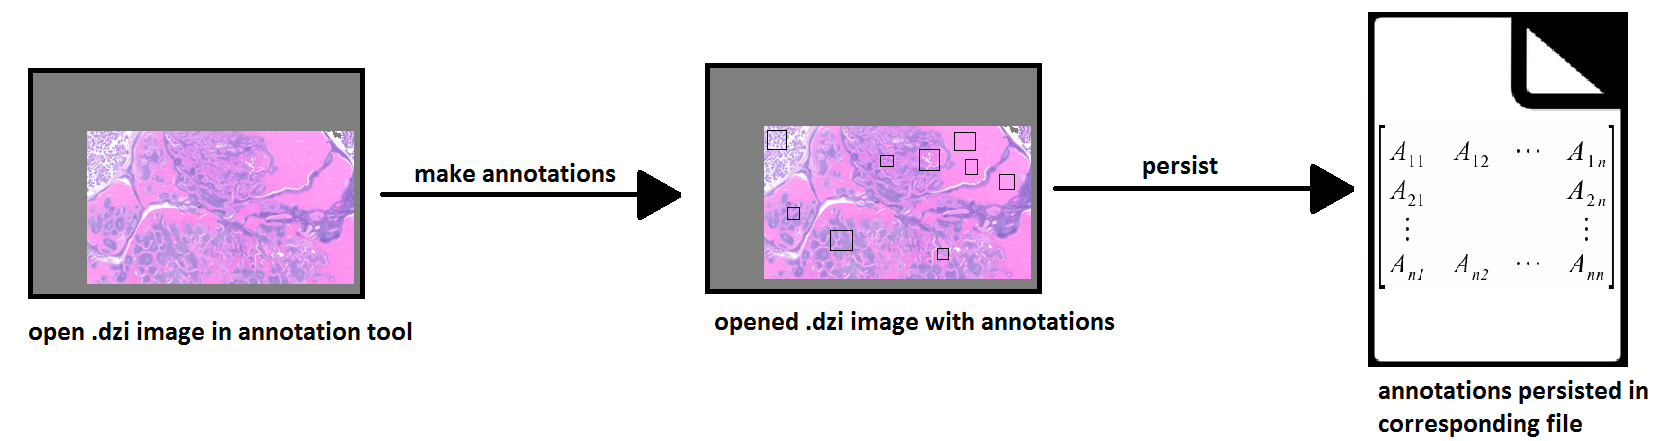
\includegraphics[scale=0.25]{img/processChainB.png}
		\caption{Visualization of the Annotation Service}
		\label{fig:fig2.4}
	\end{center}
\end{figure}

The supplied GUI will offer different tools to help the user annotate the DZI, e.g. a ruler to measure the distance between 2 points. The annotations themselves will be made via drawing a contour around an object of interest and putting a specified label to that region. To ensure uniformity of annotations, labels will not be added in free text. Instead they will be selected from a predefined dictionary.


\subsection{Tessellation Service}

The task of the Tessellation Service (TS)\nmc{TS}{Tessellation Service} is to extract annotations and their corresponding image data in such a fashion that they will become usable as training samples for NN.

\begin{figure}[H]
	\begin{center}
		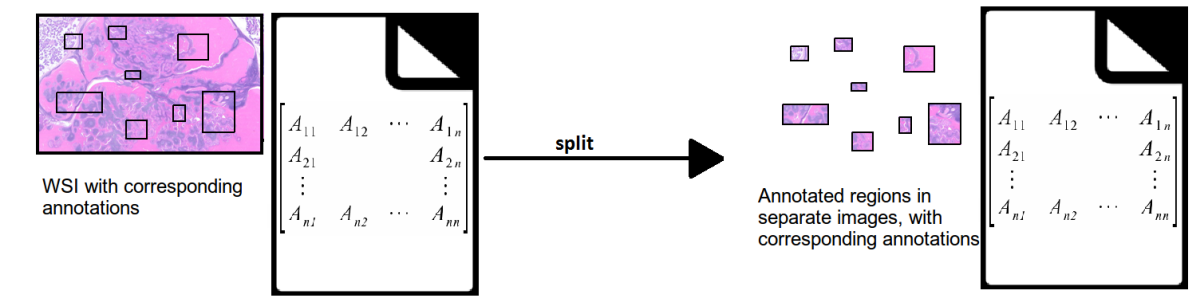
\includegraphics[scale=0.3]{img/processChainC.png}
		\caption{Visualization of the Tessellation Service}
		\label{fig:fig2.6}
	\end{center}
\end{figure}

Let there be a DZI $D$ and a corresponding set of annotations $A$. The TS will achieve the extraction by iterating over every $a_i \in A$, creating a sub-image $d_i$ which is the smallest bounding box around the region described by $a_i$ (see fig. 2.3). To be used as training sample, the TS must keep up the correspondence between $d_i$ and $a_i$.
\chapter{Conversion Service}

\section{Methodology}

The objective of the Conversion Service is to convert a given set of input WHIs into dzi files. Since a dzi is layered into a pyramid scheme, it is necessary to calculate the needed number of levels, as well as the dimensions of each level (see fig. 3.1 for an example).

\begin{figure}[H]
	\begin{center}
		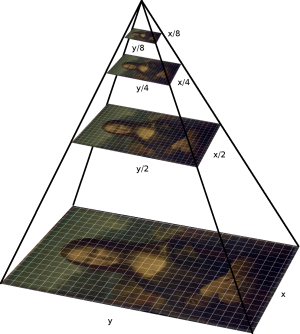
\includegraphics[scale=0.5]{img/pyramid.png}
		\caption{Example of a pyramid scheme in image processing (source: http://iipimage.sourceforge.net/images/pyramid.png)}
		\label{fig:fig3.1}
	\end{center}
\end{figure}

Therefore, the Conversion Service must be able to open an WHI $img_{input}$ of any of the in 2.2.1 defined formats. Based on the size of $img_{input}$ the number of necessary levels $lvl$ must be calculated. Once $lvl$ has been determined, $img_{input}$ must be resized into an appropriate scale for each $lvl_i$ in $lvl$. The resized image will be called $img_i$, with $i$ representing the corresponding level. In the next step, every $img_i$ will be tessellated into $x*y$ tiles. Each tile will be referrenced via $t^i_{c,r}$, with $r$ being the row and $c$ being the column of the tile in $whi_i$. To complete the conversion, the Conversion Service must create a describing xml file for each converted image $img_{dzi}$.


\subsection{Creating a Deep Zoom Image}

To create a dzi, the Conversion Service must be capable of 

\begin{table}
	\begin{center}
		\begin{tabular}{| p{3cm} | p{4cm} | p{2cm} |}
			\hline
			\textbf{option} & \textbf{description} & \textbf{image format} \\
			\hline
      		Deep Zoom Composer & dekstop app for Windows & dzi \\ \hline
      		Image Composite Editor & panoramic image stitcher from Microsoft Research for the Windows desktop & dzi \\ \hline
      		DeepZoomTools.dll & .NET-library, comes with Deep Zoom Composer & dzi \\ \hline
      		deepzoom.py & Python & dzi \\ \hline
      		deepzoom & Perl utility & dzi \\ \hline
      		PHP Deep Zoom Tools & PHP & dzi \\ \hline
      		Deepzoom & PHP & dzi \\ \hline
     		 DZT & an image slicing library and tool written in Ruby & dzi \\ \hline
     		MapTiler &  desktop app for Windows, Mac, Linux & tms \\ \hline
      		VIPS & command line tool and library for a number of languages & dzi (via dzsave feature) \\ \hline
     		Sharp & Node.js, uses VIPS & dzi \\ \hline
      		MagickSlicer & shell script (Linux/Max) & dzi \\ \hline
      		Gmap Uploader Tiler & C++ & dzi \\ \hline
      		Node.js Deep Zoom Tools & Node.js, under construction & dzi \\ \hline
      		OpenSeaDragon DZI Online Composer & Web app (and PERL and PHP scripts) & dzi \\ \hline
      		Zoomable & service, offers embeds; no explicit API & dzi \\ \hline
      		ZoomHub & service, under construction & dzi \\ \hline
      		Kakadu & C++ library to encode or decode JPEG 2000 images & iiif \\ \hline
      		PyramidIO & Java (command line and library) & dzi \\ \hline
  		\end{tabular}
  	\caption{Overview of conversion options for zooming image formats (source: \cite{web:openseadragon})}
  	\end{center}
\end{table}
  
iiif\footnote{International Image Interoperability Framework (iiif), specified by the International Image Interoperability Framework group, is an image delivery API which responds to requests via HTTP and HTTPS \cite{web:iiif}}

tms\footnote{Tile Map Service (tms) is a tile scheme developed and maintained by the Open Source Geospatial Foundation \cite{web:tms}} 


\subsection{Deepzoom.py}

Deepzoom.py\footnote{see \url{https://github.com/openzoom/deepzoom.py} for further details} is a python script and part of Open Zoom\footnote{see \url{https://github.com/openzoom} for further details}. It can either be called directly over a terminal or imported as a module in another python script. The conversion procedure itself is analogous for both methods.

If run in a terminal the call looks like the following:

\begin{lstlisting}
	$ python deepzoom.py [options] [input file]
\end{lstlisting}

The various options and their default values can be seen in tab. 3.2. If called without a designated output destination, deepzoom.py will save the converted dzi right next to the original input file.

\begin{table}[H]
	\begin{center}
		\begin{tabular}{| r | l | r |}
			\hline
			\textbf{option} & \textbf{description} & \textbf{default} \\ \hline
			-h & show help dialog & - \\ \hline
			-d & output destination & - \\ \hline
			-s & size of the tiles in pixels & 254 \\ \hline
			-f & image format of the tiles & jpg\\ \hline
			-o & overlap of the tiles in pixels (0 - 10) & 1 \\ \hline
			-q & quality of the output image (0.0 - 1.0) & 0.8 \\ \hline
			-r & type of resize filter & antialias \\ \hline
		\end{tabular}
		\caption{Options for deepzoom.py}
	\end{center}
\end{table}

The resize filter is applied to interpolate the pixels of the image when changing its size for the different levels. Supported filters are:

\begin{itemize}
	\item cubic
	\item biliniear
	\item bicubic
	\item nearest
	\item antialias
\end{itemize}

When used as module in another python script, deepzoom.py can simply be imported via the usual \emph{import} command. To actually use deepzoom.py, a Deep Zoom Image Creator needs to be created. This class will manage the conversion process:

\begin{lstlisting}[frame=single]
# Create Deep Zoom Image Creator
creator = deepzoom.ImageCreator(tile_size=[size], 
	tile_overlap=[overlap],	tile_format=[format], 
	image_quality=[quality], resize_filter=[filter])
\end{lstlisting}

The options are analogous with the terminal version (compare tab. 3.2). To start the conversion process, the following call must be made within the python script:

\begin{lstlisting}[frame=single]
# Create Deep Zoom image pyramid from source
creator.create([source], [destination])
\end{lstlisting}

Upon calling, the ImageCreator opens the input image $img_{input}$ and creates a description with all the needed information for the dzis describing xml file\footnote{compare chap. 2.1.1}. After that, the number of levels is calculated. For this, the bigger value of height and width of $img_{input}$ is chosen (see eq. 3.1) and then used to determine the number of levels $lvl$ (see eq. 3.2).

\begin{equation}
	max{\textunderscore}dim = max(height, width)
\end{equation}

\begin{equation}
	lvl = {\lceil}log_2(max{\textunderscore}dim) + 1\rceil
\end{equation}

Once $lvl$ has been determined, $img_{input}$ will be resized in the chosen quality (-q/image{\textunderscore}quality) for every level $i$, with $i \in (0, lvl-1)$. The new resolution will be calculated for both dimensions $dim$ with a function $scale$ (see eq. 3.3) analogously. Furthermore, the image will be interpolated with the specified filter (-r/resize{\textunderscore}filter). The resized image will be called $img_i$.

\begin{equation}
	scale = {\lceil}dim * 0.5^{lvl-i}\rceil
\end{equation}

Once $img_i$ has been created, it will be tessellated into as many tiles of the specified size (-s/tile{\textunderscore}size) and with the specified overlap (-o/tile{\textunderscore}overlap) as possible. Since not every image will be of the size $2^n, n \in $ in either dimension, it is highly likely that the set of tiles for the last column/row will be smaller then specified in either dimension.

Every tile will be saved as [column]{\textunderscore}[row].[format] ([format] depending on -f/file{\textunderscore}format) in a folder called according to the corresponding level $i$. This folder will be located inside another folder, called [filename]{\textunderscore}files. The describing xml file will be persisted as [filename].dzi on the same level.


\section{Implementation}

As stated before, the Conversion Service is implemented as a python script. The script is to be called inside a terminal in the following fashion:

\begin{lstlisting}
	$ python ConversionService.py -i [folder]
\end{lstlisting}

There are two possible options for the call of ConversionService.py (see tab. 3.3), it's mandatory to pick one of the two, since there are no default values.

\begin{table} [h]
	\begin{center}
		\begin{tabular}{| r | l |}
			\hline
			\textbf{option} & \textbf{description} \\ \hline
			-h & show help \\ \hline
			-i & folder with WSI to convert \\ \hline
		\end{tabular}
		\caption{Options for ConversionService.py}
	\end{center}
\end{table}

Upon calling, the \emph{main()} routine will be started, which orchestrates the whole conversion process. It looks as follows:

\begin{lstlisting}[frame=single]
def main():
	path = checkParams()
	files = os.listdir(path)
	for file in files:
		print("-----------------------------------------")
		extLen = getFileExt(file)
		if(extLen != 0):
			print("converting " + file + "...")
			convert(path, file, extLen)
			print("done!")
\end{lstlisting}

\emph{checkParams()} will check if the input parameters are valid and, if so, return the path to the specified folder or exit otherwise. In the next step, the specified folder will be checked for its content. \emph{getFileExt(file)} looks up the extension of each given file and will either return the length of the files extension, if valid (\emph{extLen} $<0$) and $0$ otherwise. Each valid file will then be converted with the \emph{convert(...)} function:

\begin{lstlisting}[frame=single]
# convert image source into .dzi format
# param path: directory of param file
# param file: file to be converted
# param extLen: length of file extension
def convert(path, file, extLen):

	if not(path.endswith("/")):
		path += "/"
	dzi = file[:extLen] + "dzi"
	
	# create Deep Zoom Image creator
	creator = deepzoom.ImageCreator(tile_size=256, tile_overlap=0,
				tile_format="png", image_quality=1.0, 
				resize_filter="bicubic")

	# create Deep Zoom image pyramid from source
	creator.create(path + file, OUTPUT + dzi)
\end{lstlisting}

The name for the new dzi file will be created from the original file name, however, the former extension will be replaced by "dzi" (see line 9). Next, deepzooms ImageCreator will be initialized with the following parameters: tile{\textunderscore}size = 256, tile{\textunderscore}overlap = 0, tile{\textunderscore}format = "png", image{\textunderscore}quality = 1.0, resize{\textunderscore}filter = "bicubic" (see line 12 - 14). Once the ImageCreator is initialized, its \emph{create(...)} function is called (see line 17), in which the input image will be converted. The output will be saved to the same folder as ConversionService.py is operating from, plus "/dzi/".


\section{Test}

Another script, \ will be deployed to make sure that the ConversionService.py is actually working correctly


\subsection{Setup}
\subsection{Result}

\chapter{Annotation Service}

\section{Objective of the Annotation Service}
As described in 2.4.2, the goal of the AS is to provide a user with the possibility to:
\begin{enumerate}[(1)]
	\item view A WSI
	\item annotate a WSI
	\item manage made annotations
\end{enumerate}

In order to achieve objective (1) - (3), a GUI needs to be deployed which supports the user in working on those tasks. (3) also adds the need for file persistence management.


\section{Methodology}
As stated in 2.1, most vendors have proprietary image formats and their own implementation of a viewer for those, thus creating a vendor lock-in. Further do vendors often only support Windows platforms, ignoring other operating systems\cite{Cornish13}\cite{DICOM10}\cite{Farahanil15}. To avoid this, a solution must be found that is independent of operating system and vendor.

Chap. 3 already established a service to convert WSIs of various formats into the DZI format, solving the problem of multiple proprietary formats. 

Independence from an operating system can be achieved by using web technologies, especially when running an application in a web browser\cite{Tseytlin14}, since those are supported by all modern operating systems. 

Because of this, the AS will be implemented as a web browser application. 


\subsection{Functionality of the Annotation Service}
The goal of viewing a WSI (1) is a straight forward task. (2) and (3) are more elusive. For that reason, this subsection elaborates on the functionality needed to help achieve those objectives.

Annotations will be created by drawing directly onto the viewed WSI. If the user spots a region of interest, a contour can be drawn around it. This can  either be done in a free hand or polygon mode. In free hand mode, the contour will follow the mouse pointer until the mode is disabled again, all the while drawing a contour. Upon deactivation, the contour will be closed. In polygon mode, the user can place coordinates which will be connected from one to another in the order they're placed in. A contour in this mode considers to be closed, once a point on the contour is clicked a second time.


% draw free hand or draw polygon
% set poi
% measure distance
% create dictionaries
% activate differnt dictionaries
% add labels to dictionaries
% select labels
% why dictionaries and labels can only be deleted by manipulating the file on the server, but regions can be deleted?
% regions and context regions


\subsection{Parts of the Annotation Service}
The AS is implemented in 2 parts. Those are the Annotation Service Server (ASS)\nmc{ASS}{Annoation Service Server} and the Annotation Service Viewer (ASV)\nmc{ASV}{Annotation Service Viewer}.

This is because of the \emph{same-origin policy} (SOP)\nmc{SOP}{same-origin policy}. SOP is a security concept of the web application security model. It prevents a direct access to files, if the parent directory of the originating file is not an ancestor directory of the target file\cite{web:mdn}. Because of the SOP, WSIs would have to be located in the directory structure of the AS, which by itself doesn't create a problem. To get a new WSI there, however, the user would be forced to navigate through the structure of the AS, find the correct directory and then place it there manually. This makes knowledge of the service structure necessary and creates a horrible UX. Furthermore, tinkering with the file structure of the AS creates a possible source for errors.

A workaround of this problem is to deploy a web server, which can redirect the image request, access the WSI and return it in response\cite{Tseytlin14}. The use of DZI creates another advantage: the used image pyramid model reduces the network traffic necessary to load and show a WSI in a viewer\cite{Cornish13}\cite{DICOM10}.

Furthermore, even a single WSI takes up a lot of storage capacity\cite{Singh11}. Having multiple WSIs on a local hard drive would either create the need for huge amounts of available storage space or restrict the amount of accessible WSIs to a few at any given time. The latter solution would create two follow-up problems:
\begin{itemize}
	\item WSIs are medical images and as such confidential information. Therefore, not everyone is allowed to just have access to or copies of them\cite{COA}\cite{USSanDiego}. Once a copy of a WSI changes hands, it is virtually impossible to make sure that privacy regulations will be uphold.	
	\item With only a small amount out of all WSIs accessible at all times, the need for copying files back and forth arises as soon as the user wants to compare, update or correct a WSI, which is not on his local file system at the given moment. Not only is this a great source for possible errors, but also very time consuming and inefficient.
\end{itemize}

With the use of a web server as a central image repository, WSIs and the access to them can be managed in a centralized spot, while upholding confidentiality regulations. Furthermore, a user has access to all of her/his WSIs at any given time, without the need for creating subsets and copying files back and forth. Depending on the setup of the network, other factors can come into play as well. Access to and sharing of rare cases, educational material and training samples can be granted without a complicated distribution chain and a smaller risk for confidentiality issues. It also enables the consultation of case experts independent of their physical position on the planet\cite{Wilbur09}.


\subsubsection{Annotation Service Server}
The ASS has 2 main purposes.

First, it serves as a so called \emph{Digital Slide Repository} (DSR)\nmc{DSR}{Digital Slide Repository}. A DSR manages storage of WSIs and their metadata. Furthermore, it serves requested image data to a viewer client, such as the ASV\cite{Cornish13}. 

Second, it is responsible for file management. In detail, this means:
\begin{itemize}
	\item persist made annotations in a file
	\item deliver annotation data together with image data
	\item serve list of all available label dictionaries
	\item serve label dictionary entries
	\item save added entries to existing label dictionary
	\item create new label dictionaries
\end{itemize}




% local for now


\subsubsection{Annotation Service Viewer}
To enable the pathologist to view a WSI and annotate it, a GUI needs to be deployed. This GUI will be called Annotation Service Viewer and developed in an iterative approach with the help of selected pathologists. After each iteration, the GUI and user experience (UX)\nmc{UX}{User Experience} will be evaluated. This way, the ASV can be adapted to the needs of a real life environment based on the pathologists feedback.

\begin{figure}[H]
	\begin{center}
		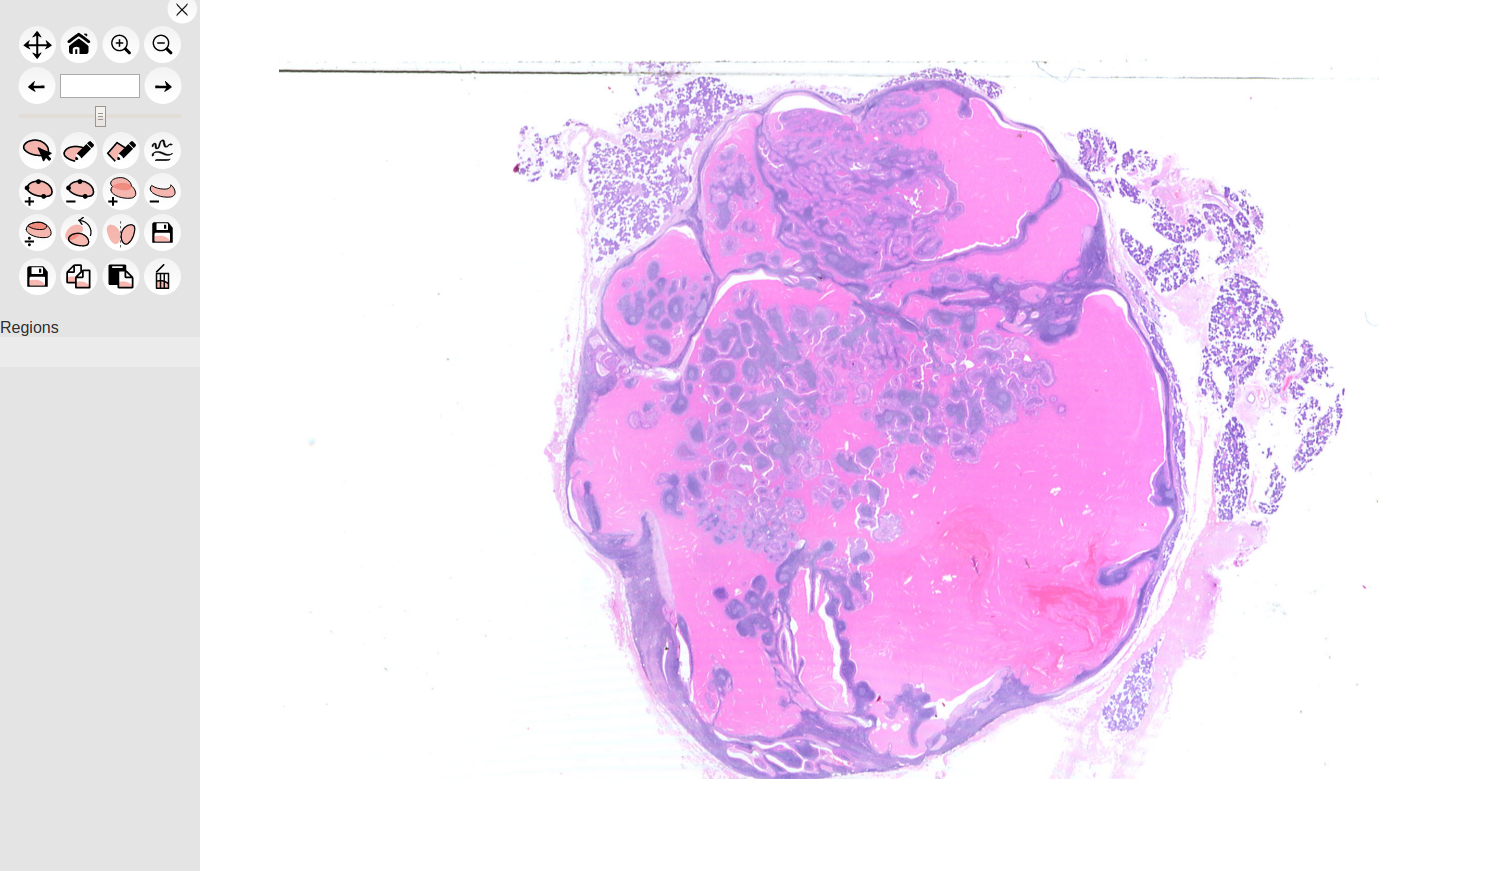
\includegraphics[scale=0.2]{img/microdrawUI.png}
		\caption{Microdraw GUI with opened WSI}
		\label{fig4_microdrawUI}
	\end{center}
\end{figure}

The first iteration of the ASV will be based on an open source project called \emph{MicroDraw}\footnote{See \url{https://github.com/r03ert0/microdraw} for more information on the MicroDraw project} (see fig. \ref{fig4_microdrawUI} for MicroDraws GUI).  MicroDraw is a web application to view and annotate \emph{"high resolution histology data"}\cite{web:microdraw2}. The visualization is based on another open source project, called \emph{OpenSeadragon}\cite{web:openseadragon}. Annotations are made possible by the use of \emph{Paper.js}\footnote{see \url{http://paperjs.org/} for more information on Paper.js}. Apart from the frameworks used, MicroDraw is written in JavaScript using HTML5, CSS3 and jQuery\footnote{see \url{https://jquery.com/} for more information on jQuery}.


\section{Implementation}
% what was used for implementation
\subsection{Technologies and Frameworks}
% openslide, openslide web server
% python web server, flask, openslide, java script, html5, css, jquery
\subsection{Annotation Service Viewer}
% documentation
\subsection{Annotation Service Server}
% documentation
\chapter{Tessellation Service}

\section{Objective of the Tessellation Service}
\label{sec5_objective}
The objective of the TS is to provide a service that extracts image regions annotated by the AS to create samples for the training of a NN\footnote{
	Compare subsection \ref{sec2_learning}
}. In this context, "extraction" describes the process of creating sub images of the original image, which contain all of the annotated ROI and as little of anything else as possible. Additionally, the correspondence with the associated region label must be kept. The AS uses \emph{regions}\footnote{
	Compare subsection \ref{sec4_region}
} to describe ROIs. Those regions are persisted in a JSON file.

Therefore, the TS has 2 objectives:
\begin{enumerate}[(1)]
	\item parse a JSON file and acquire its region data
	\item extract ROIs based on the acquired region data
\end{enumerate}


\section{Methodology}
\label{sec5_method}
The objective of the TS is to create usable training samples for NNs, as stated in section \ref{sec5_objective}. Depending on the setup, chosen learning method\footnote{
	Compare section \ref{sec2_introNN}
} and purpose of the NN, the requirements imposed on the training samples may vary. Smith demonstrates in \cite{Smith97} exemplary how to train a NN to recognize letters in images of written text by training it with 10x10 pixel grayscale images (256 gray levels/pixel) of letters. Shereena and David introduce a novel content based image retrieval classification method in \cite{Shereena14}, based on color and texture features. Other approaches extract features through the use of mathematical models from the supplied images (such as edges or shapes)\cite{Harvey91}.

Because of those varying requirements, the TS will be capable of producing different output:
\begin{enumerate}[(1)]
	\item Unaltered image of ROI
	\item Resize images to a specific width and height
	\item Approximate ROIs via tessellation
	\item Convert extracted images to grayscale
\end{enumerate}

A user can draw a region's path without any restrictions concerning the pattern, resulting in ROIs that can be of arbitrary shape. Therefore, bounding boxes (BB)\nmc{BB}{Bounding Box}\footnote{
	A BB is a rectangular body, fully enclosing a provided (two dimensional) object of arbitrary shape\cite{Toussaint83}.
} are used for ROI extraction in the cases (1) and (2) (see fig. \ref{fig5_bbExample} for an example).

\begin{figure}[H]
	\begin{center}
		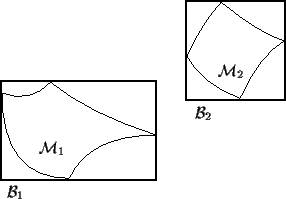
\includegraphics[scale=0.6]{img/bb1.png}
		\caption{Examplary BBs: $B_1$ is BB of $M_1$, $B_2$ is BB of $M_2$ (source: \url{http://www.idav.ucdavis.edu/education/GraphicsNotes/Bounding-Box/Bounding-Box.html})}
		\label{fig5_bbExample}
	\end{center}
\end{figure}

In the case of (1), an ROI's BB is copied pixel by pixel into a new image. The resizing (scaling the output image up or down to the provided pixel values) in the case of (2) makes preprocessing of the BB necessary. This has 2 reasons:
\begin{itemize}
	\item If the aspect ration of the provided width and height is different than the one of the BB, the resulting image will be distorted.
	\item When scaling images down, interpolation can be used, to reduce the information loss of the image\cite{Thevanez00}. This is partially possible when scaling images up as well, e.g. via fractal interpolation, but a non trivial task\cite{Guerdri16}.
\end{itemize}

Therefore, the size of the BB will be adjusted to match the aspect ratio of the provided width and height. If the resulting BB is bigger then the provided width and height, the image will be scaled down and interpolated. If the BB is smaller, it will be scaled up instead of the image. This leads to a bigger area inside the BB that is not part of the ROI, but a pixel ratio of 1:1 between original and extracted image, resulting in no distortion or loss of quality.

Case (3) approximates a ROI by tessellating\footnote{
	\emph{Tessellation} describes the tiling of a plane using one or more geometric shapes with no overlaps or gaps\cite{Clifford09}.
} it into tiles of the provided width and height (see fig. \ref{fig5_tesExample} for an example). Every tile inside the region's enclosing path (or touched by it) is targeted by the extraction. Each tile is extracted into an individual image.

\begin{figure}[H]
	\begin{center}
		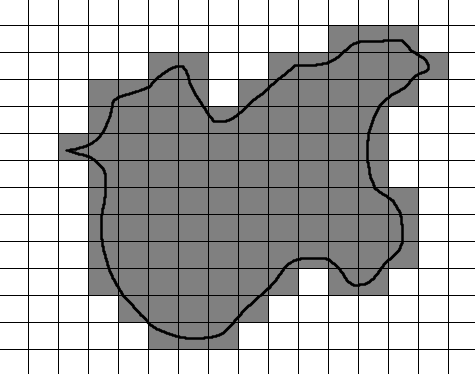
\includegraphics[scale=0.5]{img/tessellation.png}
		\caption{Example of an ROI approximated via tessellation (gray tiles belong to the ROI)}
		\label{fig5_tesExample}
	\end{center}
\end{figure}

Cases (1) - (3) can be combined with (4) to convert the extracted ROI images into grayscale images.

A region contains additional information besides the label that can be utilized, especially the level of magnification\footnote{
	Compare subsection \ref{sec4_region}
}. As Doyle has shown in \cite{Doyle10}, the level of magnification an annotation was made in is an important factor. This is due to the fact that manual annotations made in lower magnifications do not have the granularity needed for higher ones, which results in numerous false positives and negatives and therefore distorts the ground truth\cite{Janowczyk16}. A region's zoom attribute informs at what level of magnification a region was drawn in, thus helping to assess the described issue.

To utilize the additional metadata, each extracted region will also have a corresponding metadata file. This metadata contains:
\begin{itemize}
	\item the name of the extracted image file (case (1) and (2)), or a list of all image tiles which belong to the ROI (case (3))
	\item the region's label
	\item the level of magnification
	\item the region's context
\end{itemize}

Section \ref{sec5_objective} additionally stated the objective of keeping up correspondence between an ROI and its associated label. To achieve this, an extracted image will be saved in a directory of the same name as its corresponding label. This way, all ROIs of a specific label can be collected in one location. Additionally, the corresponding metadata file will contain an association between image file and label name.


\section{Implementation}
\label{sec5_impl}
The TS is implemented as a python script called \textbf{\emph{TessellationService.py}}\footnote{
	See its GitHub repository for more information: \url{https://github.com/SasNaw/TessellationService}.
}. As stated in sections \ref{sec5_objective} and \ref{sec5_method}, its purpose is to extract annotated ROIs from a WSI. This is done with the help of the following frameworks and libraries: \emph{OpenSlide}, \emph{NumPy}, \emph{Pillow} and \emph{OpenCV} (Open Source Computer Vision Library)\nmc{OpenCV}{Open Source Computer Vision Library}.

\emph{OpenSlide} was used to access and read a provided WSI\footnote {
	Compare subsection \ref{sec4_asvFrameworks} - OpenSlide
}.

NumPy is a python library for efficient scientific computing, especially regarding operations involving multi-dimensional array objects\cite{Walt11}. Since a lot of image operations are based on the use of matrices, this library was used to increase efficiency.

OpenCV is an open source computer vision and machine learning software library. It was built to provide a common infrastructure for computer vision applications. It offers numerous functions regarding image processing and machine learning, with a strong focus on real-time computing and efficiency\cite{Bradski08}. Its main purpose in the TS is to create a reference image for the tessellation function\footnote{
	See subsection \ref{sec5_tessellation}
}

Pillow is an imaging library, which offers methods to read from and write to images. It was used for reading, writing, scaling and converting the extracted images.

A detailed documentation of the TS' functions can be found in appendix \ref{secC}.

\subsection{Execution}

The TS can be called over the python interpreter:

\begin{lstlisting}
	$ python TessellationService [input] [dictionary] [params]
\end{lstlisting}

The files which are supposed to be targeted by the extraction process are handed to the TS via the \emph{[input]} argument. This can be a list of WSIs, DZIs and directories. If a directory is handed to the TS, all subdirectories (except a DZI's \emph{"{\textunderscore}files"} directory) will be searched as well.

As mentioned in chapter \ref{sec4_as}, multiple dictionaries can be used for annotation. Since every WSI has an individual save file for each dictionary (compare subsection \ref{sec4_setup}), it is necessary to provide the dictionary targeted for extraction via the [dictionary] parameter. Each input file must have its associated save file in the same directory.

[input] and [dictionary] are mandatory arguments.

As mentioned in section \ref{sec5_method}, it might be necessary to create different output images for different purposes. Therefore, the TS has a list of optional parameters to manipulate the created output in order to be applicable to a wider variety of cases (see tab. \ref{tab5_tsParams}). Those parameters are optional. 

\begin{table}[H]
	\begin{center}
		\begin{tabular}{| p{3cm} | p{5cm} | p{3cm} |}
			\hline
			\textbf{name} & \textbf{description} & \textbf{default}\\ \hline
			-h, --help & show help & - \\ \hline
			-f, --force-overwrite & flag to overwrite images with the same name (if not supplied, a number will be added to the image name) & false \\ \hline
			-g, --grayscale & flag to convert images to grayscale images before saving them & false \\ \hline
			-i, --interpolation & choose interpolation method: nearest neighbor, bilinear, bicubic, lanczos  & nearest neighbor interpolation \\ \hline
			-o, --output [directory] & choose output directory (if not provided, the TS will save all extracted images in its own directory) & - \\ \hline
			-r, --resize [width] [height] & resize all output images to the provided [width] and [height] in pixel & - \\ \hline
			-s, --show-tessellated & flag to create window and show stitched image resulting from the tessellation process (only for debugging purposes, see \emph{"-t"}) & false\\ \hline
			-t, --tessellate [width] [height] & tessellate regions into tiles of the provided [width] and [height] in pixels & - \\ \hline
		\end{tabular}
		\caption{Optional parameters for the TS}
		\label{tab5_tsParams}
	\end{center}
\end{table}


\subsection{Extraction process}

The TS receives a list of files and folders to extract regions from and iterates over each entry. If the entry is a directory, each contained element will be checked for its type. If it is a WSI/DZI file, the extraction is started right away. Once the extraction is finished, the next element is examined. If the entry is a directory, each contained element is subject to the same evaluation. WSI/DZI files are extracted, while subdirectories are recursively traversed until the end of the directory tree. Each element found in this process that qualifies for region extraction is extracted. Fig. \ref{fig5_tsRunUml} visualizes the described process in an activity diagram.

\begin{figure}[H]
	\begin{center}
		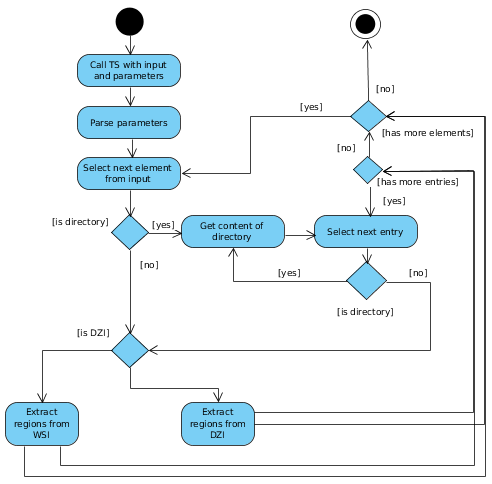
\includegraphics[scale=0.6]{img/ts_run.png}
		\caption{Activity diagram of TS' extraction procedure}
		\label{fig5_tsRunUml}
	\end{center}
\end{figure}

OpenSlide is used to read a provided WSI. Since OpenSlide can not open a native DZI, but only wrap an OpenSlide object into a DZG\footnote{
	Compare subsection \ref{sec4_openslide}
}, a different approach had to be chosen to access a provided DZI.

Both approaches share the following utility functions\footnote{
	See appendix \ref{secC} for documentation of the individual function's source code.
}:

\begin{itemize}
	\item \texttt{read{\textunderscore}json(path)} tries to read the JSON file at the provided path. If successful, it returns a list with the regions parsed from the file. If the file was not found or corrupt, a message will be printed on the terminal, informing the user about the exception.
	
	\item \texttt{save{\textunderscore}image(image, region, slide{\textunderscore}name, *tiles)} generates an appropriate name from the region information and the slide{\textunderscore}name for the image and metadata file. The name differs between tessellated and non-tessellated output (see tab. \ref{tab5_outputNames}).
	
	If -r is provided, the image will be resized to the supplied height and width, with the interpolation method provided via -i (default: nearest neighbor interpolation). If -g is specified, the image will be converted to grayscale with the luma transform defined in the ITU-R 601-2 standard\cite{ITUR94} (see eq. \ref{eq:luma}).
	\begin{equation}\label{eq:luma}
		L = R * 299/1000 + G * 587/1000 + B * 114/1000
	\end{equation}
	
	Eq. \ref{eq:luma} averages out the RGB values of every pixel under consideration of how a human eye perceives colors.
	
	If -o was provided, the processed image will be saved in the supplied location inside a directory with the name of the extracted region's label.
	
	\item \texttt{save{\textunderscore}metadata(name, region, *tiles)} writes the corresponding metadata to an extracted image into a file (see tab. \ref{tab5_outputNames} for the file name pattern). The metadata is a JSON map and contains the values listed in tab. \ref{tab5_metadataJson}. When the TS is run with -t, the \emph{"image"} key is replaced by \emph{"tiles"}, which contains a JSON list with the names of all tiles belonging to the extracted image (each individual image name is according to the pattern in tab. \ref{tab5_outputNames}).
	
	\begin{table}[H]
		\begin{center}
			\begin{tabular}{| l | p{6cm} | l |}
				\hline
				\textbf{key} & \textbf{value} & \textbf{type}\\ \hline
				context & the image region's context & JSON list\\ \hline
				image & name of the extracted image file (compare tab. \ref{tab5_outputNames}) & string \\ \hline
				label & the region's label & string\\ \hline
				zoom & the region's zoom & float\\ \hline
			\end{tabular}
			\caption{File name patterns of generated output}
			\label{tab5_metadataJson}
		\end{center}
	\end{table}
	
	\item \texttt{get{\textunderscore}bounding{\textunderscore}box(region)} iterates over every segment of a region's path and builds the BB by collecting the minimal and maximal values for x and y (compare fig. \ref{fig5_bbExample}).
	
	\item \texttt{resize{\textunderscore}bounding{\textunderscore}box(bounding{\textunderscore}box)} is used to adjust a region's BB to a different aspect ratio. This is to avoid image distortion when the -r parameter specifies a different image ratio than the BB's inherent one (see fig. \ref{fig5_resizeBBexample} for an example).
	
	\begin{figure}[H]	
		\begin{center}
			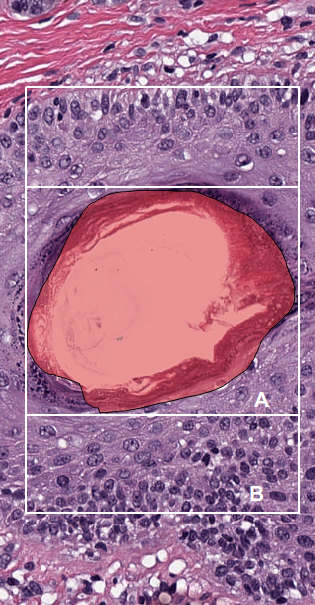
\includegraphics[scale=0.3]{img/bbResizeExample.png}
			\caption{Example for adjusted BB (A - original BB with aspect ratio of $\sim$1:1, B - adjusted BB to aspect ratio of $\sim$1:2)}
			\label{fig5_resizeBBexample}
		\end{center}
	\end{figure}
	
	\item \texttt{scale{\textunderscore}bounding{\textunderscore}box(bounding{\textunderscore}box, scale)} scales a BB by a provided scale. This is to avoid image distortions due to scaling images up (compare section \ref{sec5_method}). While \texttt{get{\textunderscore}bounding{\textunderscore}box(region)} changes the aspect ratio of a BB, \texttt{scale{\textunderscore}bounding{\textunderscore}box(bounding{\textunderscore}box, scale)} keeps the aspect ratio and changes the BB as a whole instead.
\end{itemize}

\begin{table}[H]
	\begin{center}
		\begin{tabular}{| p{3cm} |p{4cm} | p{4cm} |}
			\hline
			\textbf{name} & \textbf{image file} & \textbf{metadata file}\\ \hline
			\textbf{-t not provided} & [slide{\textunderscore}name]{\textunderscore}[region.uid].{\newline}jpeg & [slide{\textunderscore}name]{\textunderscore}[region.uid].{\newline}metadata.json \\ \hline
			\textbf{-t provided}  & [slide{\textunderscore}name]{\textunderscore}[region.uid]\newline([row]{\textunderscore}[column]).jpeg & [slide{\textunderscore}name]{\textunderscore}[region.uid].{\newline}metadata.tessellated.json \\ \hline
		\end{tabular}
		\caption{File name patterns of generated output}
		\label{tab5_outputNames}
	\end{center}
\end{table}


\subsection{Extraction without Tessellation}
\label{sec5_extraction}
As mentioned above, the implementation of the conversion differs for WSI and DZI due to the role of OpenSlide in the extraction of WSIs. The following two sections describe the extraction process for both cases.

\subsubsection{WSI}
The WSI extraction process is done in the \texttt{wsi(file)} function\footnote{
	See appendix \ref{secC} for a function documentation.
}. It opens the provided file via OpenSlide, builds a name from its path and parses the regions of the WSI via \texttt{read{\textunderscore}json(path)}. The function iterates over every parsed region to extract it. The extraction process is visualized in fig. \ref{fig5_tsWsiUml}. 

\begin{figure}[H]
	\begin{center}
		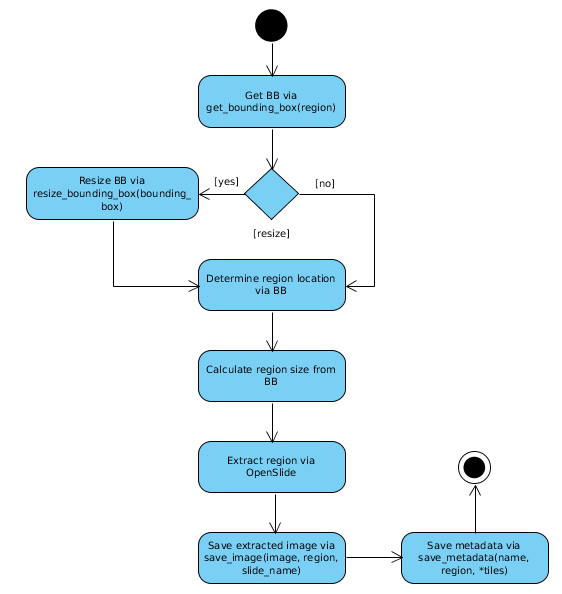
\includegraphics[scale=0.45]{img/ts_wsi_uml.png}
		\caption{Activity diagram of TS' WSI extraction (without tessellation)}
		\label{fig5_tsWsiUml}
	\end{center}
\end{figure}

As shown in fig. \ref{fig5_tsWsiUml}, calculating the BB is the first step. To do so, the \texttt{get{\textunderscore}bounding{\textunderscore}box(region)} function is used, which returns a python dictionary with the minimum and maximum values of x and y in the associated region's path. If -r was provided, the BB's size will be adjusted to fit the supplied image ratio.

Next, the location of the region is determined. This is done by taking the minimum value for x and y from the BB and declaring it as upper, left corner of the region. The size is calculated by subtracting the minimum from the maximum value for x and y respectively (see eq. \ref{eq:sizeX} and \ref{eq:sizey}).

\begin{equation}\label{eq:sizeX}
size_x = BB_{max(x)} - BB_{min(x)}
\end{equation}
\begin{equation}\label{eq:sizey}
size_y = BB_{max(y)} - BB_{min(y)}
\end{equation}

OpenSlide's \texttt{readRegion(location, level, size)} function is used to retrieve the region in a separate image from the original baseline image. This extracted image is then written into a file, together with its associated region's metadata.

\subsubsection{DZI}
Since it is not possible to open a DZI with OpenSlide, the extraction process for DZI differs from the one for WSI. It is implemented in the \texttt{dzi(file)} function\footnote{
	See appendix \ref{secC} for a function documentation.
}, which starts and manages the extraction process. Since an image must be stitched together manually, the information about tile size and image dimensions must be parsed from the DZI metadata file, as well as the level containing the baseline image (since DZI uses n instead of 0 for the level with the highest resolution). Once the information is parsed, a file name is created from the file path and the corresponding regions are parsed from the associated JSON file. Fig. \ref{fig5_tsDziUml} visualizes the extraction process and its individual steps, which are executed for each region.

\begin{figure}[!h]
	\begin{center}
		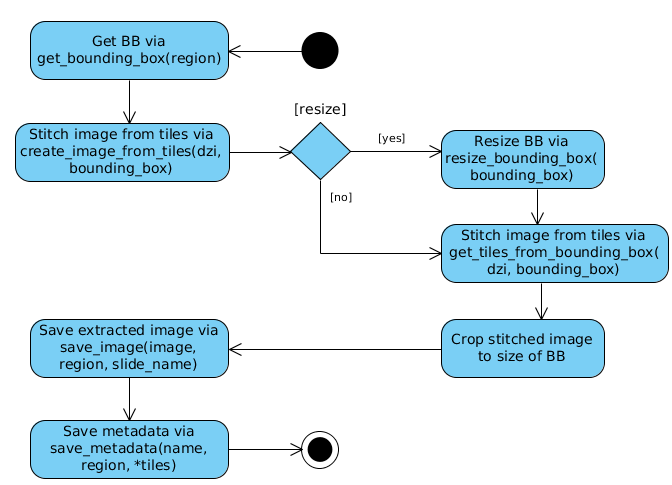
\includegraphics[scale=0.45]{img/ts_dzi_uml.png}
		\caption{Activity diagram of TS' DZI extraction (without tessellation)}
		\label{fig5_tsDziUml}
	\end{center}
\end{figure}

The BB is created via the \texttt{get{\textunderscore}bounding{\textunderscore}box(region)} function. Once the BB is created, the stitching process of the area covered by the baseline image begins. This is realized in the \texttt{create{\textunderscore}image{\textunderscore}from{\textunderscore}tiles(dzi, bounding{\textunderscore}box)} function. It first checks, if the -r parameter was provided and if so, if the aspect ratio of the BB matches the ratio of the supplied height and width. If necessary, the BB is adjusted via \texttt{resize{\textunderscore}bounding{\textunderscore}box(bounding{\textunderscore}box)}.
 
The first step in stitching the baseline image area together, is determining the size of the BB (see eq. \ref{eq:sizeX} and \ref{eq:sizey}). To determine the needed tiles, $BB_{min(x)}$, $BB_{min(y)}$, $BB_{max(x)}$ and $BB_{max(y)}$ are divided by the DZI's tile size, resulting in $BB_{min(x)}^t$, $BB_{min(y)}^t$, $BB_{max(x)}^t$ and $BB_{max(y)}^t$. Those values are then iterated from the pair $(BB_{min(x)}^t, BB_{min(y)}^t)$ to $(BB_{max(x)}^t, BB_{max(y)}^t)$. Each of the resulting pairs $(BB_x^t, BB_y^t)$ refers to a tile from the baseline image. The baseline image area is stitched together by iterating over all pairs $(BB_x^t, BB_y^t)$ and stitching the corresponding tiles together. This is implemented in the \texttt{get{\textunderscore}image{\textunderscore}from{\textunderscore}bounding{\textunderscore}box(dzi, bounding{\textunderscore}box)} function. The stitched image is then cropped to fit the size and position of the BB and saved together with its corresponding metadata file (via \texttt{save{\textunderscore}file(image, region, slide{\textunderscore}name)} and \texttt{save{\textunderscore}metadata(name, region, *tiles)}).


\subsection{Extraction with Tessellation}
\label{sec5_tessellation}

If a region is extracted with the -t parameter (compare tab. \ref{tab5_tsParams}), it will be tessellated into multiple image tiles of provided width and height (compare \ref{sec5_method}(3) and fig. \ref{fig5_tesExample}). As in subsection \ref{sec5_extraction}, the main difference between the processing of a WSI and a DZI is the need to parse the DZI's associated metadata and stitch an area of the baseline image. With that exception, the tessellated extraction works identical in both cases.

The baseline image is tessellated into $m$*$n$ virtual tiles (see eq. \ref{eq:m} and \ref{eq:n}). All virtual tiles containing parts of the region's path are saved in a list $L^{path}$.
\begin{equation}\label{eq:m}
	m = \text{baseline image height} / \text{tile height}
\end{equation}
\begin{equation}\label{eq:n}
	n = \text{baseline image width} / \text{tile width}
\end{equation}

The virtual tiles are needed to create and work with the \emph{reference image} (RI\nmc{RI}{Reference Image}). The RI is a central component of the tessellated extraction process. It is a binary image, which is $m$ pixels high and $n$ pixels wide. Each pixel represents a virtual tile of the baseline image. If a pixel is white, the corresponding virtual tile is part of the region to extract.The RI is a matrix representation of which tile is needed from the baseline image (see fig. \ref{fig5_riExample}).

\begin{figure}[!h]
	\begin{center}
		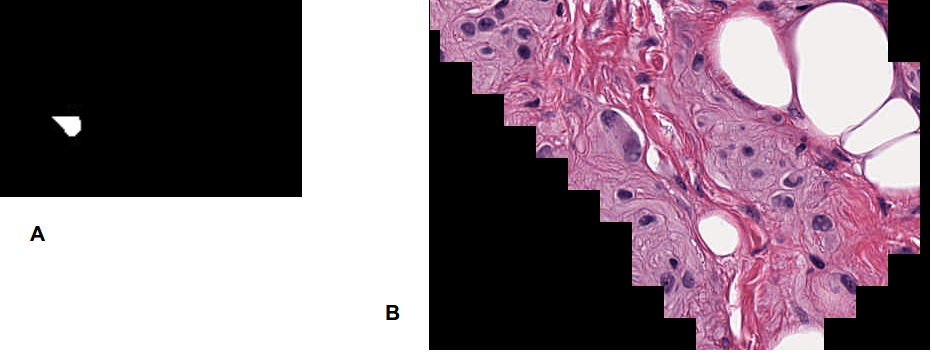
\includegraphics[scale=0.35]{img/RI_example.png}
		\caption{Example of RI (A) and resulting image tiles (B, stitched) with a tile size of 32x32 pixel (example was created using CMU-1.svs from Aperio, see appendix \ref{secA})}
		\label{fig5_riExample}
	\end{center}
\end{figure}

When created, the RI has only black pixels. To color the pixels associated with the ROI white,  OpenCV's \texttt{drawContours(image, contours, color, fill)} function is used. Since the correspondence of pixels and tiles is bidirectional, $L^{path}$ can be used to describe the contour. The drawn contour is then filled white.

The last step is to iterate each pixel of the RI. For every white pixel found, the corresponding tile is extracted from the baseline image and saved into an individual image file (compare tab. \ref{tab5_outputNames} for the naming convention).


\section{Test}
\subsection{Setup}
\subsection{Result}
\chapter{Conclusion}

\section{Results}
The research goal of this thesis was to create a set of tools which enables deep learning and pathology experts to cooperate in creating a ground truth for NN by annotating WSIs. 3 objectives were defined to reach that goal\footnote{
	Compare section \ref{sec1_researchObjective}	
}:

\begin{enumerate}[(1)]
	\item The introduction of a conversion tool, which turns proprietary WSI formats into an open one.
	\item The deployment of a WSI viewer tool with annotation capabilities and easy-to-understand GUI.
	\item The implementation of a tool that is capable of turning persisted annotations into a format usable as ground truth.
\end{enumerate}

Each objective has a corresponding chapter, in which one or more tools were introduced. The tools, chapters and goals correspond as stated in tab. \ref{tab6_objCorrespondence}.

\begin{table}[H]
	\begin{center}
		\begin{tabular}{| R{2cm} | R{1.5cm} | p{3cm} | p{4cm} |}
			\hline
			\textbf{objective} & \textbf{chapter} & \textbf{tool} & \textbf{repository} \\ \hline
			(1) & \ref{sec3_cs} & ConversionService.py & \url{https://github.com/SasNaw/ConversionService} \\ \hline
			(2) & \ref{sec4_as} & ASS \& ASV & \url{https://github.com/SasNaw/AnnotationService} \\ \hline
			(3) & \ref{sec5} & ConversionService.py & \url{https://github.com/SasNaw/TessellationService} \\ \hline
		\end{tabular}
		\caption{Correspondence of objectives, chapters and tools}
		\label{tab6_objCorrespondence}
	\end{center}
\end{table}

Chapter \ref{sec3_cs} introduced the CS, which is capable of converting a proprietary WSI to a DZI. A test was set up to ensure its functionality, which was successful (compare subsection \ref{sec3_test}).

Chapter \ref{sec4_as} introduced the AS, which consists of the ASS and the ASV. It was developed in an iterative process with regular feedback after each iteration from a pathologist concerning the GUI and UX. The ASS' use of OpenSlide enabled the AS to read and view a proprietary WSI, thus making the CS redundant.

Chapter \ref{sec5} introduced the TS, which extracts annotations made and persisted by the AS into individual images with a corresponding metadata file, thus delivering a ground truth for the training of NN. To ensure, that the TS works as intended, a test case was set up (compare subsection \ref{sec5_test}), which was completed successfully.


\section{Conclusion}

Objective (1), the conversion of proprietary to open image formats, was accomplished by the CS. The need of converting a WSI to DZI prior to using it in the AS was inflexible and cumbersome. Thus, an on demand conversion was implemented into the AS, which eliminates the need of a prior conversion and enabled the AS to view a proprietary WSI directly.
 
Objective (2), developing a WSI viewer with annotation capabilities\footnote{
	Compare subsection \ref{sec4_asvPart}
}, was accomplished by the AS, which consists of 2 parts: ASS and ASV. The ASS delivers a local slide repository. Additionally, it offers a RESTful API, which can be used by the ASV to request and persist data. Since the ASV is running in a web browser, it can be used independent of an operating system. The ASV offers a simple GUI to make annotations to a WSI based on regions\footnote{
	Compare subsection \ref{sec4_region}
} and label dictionaries.

Objective (3), the extraction of the AS' annotations to create a ground truth, was accomplished by the TS. It offers a python script to extract an ROI out of a WSI into an individual image, while keeping correspondence to the region's label and metadata through the use of directory structure and metadata files.

The tools presented in this thesis are capable of handling the complete process chain introduced in subsection \ref{sec2_pc}. Thus, the goal of introducing tools for the cooperative annotation of WSIs by deep learning and pathology experts to create a ground truth was accomplished.



\section{Future work}
% turn ASS into a real server
% deliver a working segmentation script
% implement wsi browser
% implement wsi stack in viewer?
% integrate CS and TS into ASV
% visualization of tessellation in ASV
\begin{appendices}
	\chapter{Test Data}

\section{Files on disc}
\label{secA_cd}

A disc is included at the end of this thesis. This disc contains the 3 introduced services from the chapters \ref{sec3_cs} (CS), \ref{sec4_as} (AS) and \ref{sec5} (TS). Alternatively, they are available at their corresponding GitHub repositories (see tab. \ref{tabA_paths}).

\begin{table}[H]
	\begin{center}
		\begin{tabular}{| p{1.5cm} | p{4.5cm} | p{5cm} |}
			\hline
			\textbf{service} & \textbf{disc path} & \textbf{GitHub repository} \\ \hline
			CS & /services/ConversionService & \url{https://github.com/SasNaw/ConversionService} \\ \hline
			AS & /services/AnnotationService & \url{https://github.com/SasNaw/AnnotationService} \\ \hline
			TS & /services/TessellationService & \url{https://github.com/SasNaw/TessellationService}  \\ \hline
		\end{tabular}
		\caption{Services with their disc paths and repository URLs}
		\label{tabA_paths}
	\end{center}
\end{table}

All tools presented in this thesis are open source and their use, further development and diversification are highly encouraged.

The disc also contains 2 exemplary WSI files (CMU-1.svs from Aperio, see \ref{sec_A1} and CMU-3.ndpi from Hamamatsu, \ref{secA_Hama}). Due to the limited storage space available on the medium and the size of most WSI files, only 2 could be provided on disc. They can be found under \emph{/testdata/wsi/} and are usable for all 3 services.

The JSON save file from \ref{sec5_test} can also be found on the disc, at \emph{/testdata/json/CMU-1.svs{\textunderscore}example.json}.



\section{Free Whole Slide Images}
\label{secA}
The following test data was used for all tests involving CS, AS and TS. It can be found at OpenSlide's homepage, at the freely distributable test data section\footnote{
	See \url{http://openslide.cs.cmu.edu/download/openslide-testdata/} for more information.
}. Various slides can be found there. The sections \ref{sec_A1} - \ref{sec_A8} give listings of all used WSIs, sorted by vendor and file format.

\subsection{Aperio (.svs)}
\label{sec_A1}

\begin{table}[H]
	\begin{center}
		\begin{tabular}{| p{4cm} | p{2cm} | p{5cm} |}
			\hline
			\textbf{name} & \textbf{size (MB)} & \textbf{description} \\ \hline
			CMU-1-JP2K-33005.svs & 126.42 & Export of CMU-1.svs, brightfield, JPEG 2000, RGB\\ \hline
			CMU-1-Small-Region.svs & 1.85 & Exported region from CMU-1.svs, brightfield, JPEG, small enough to have a single pyramid level \\ \hline
			CMU-1.svs & 169.33 & Brightfield, JPEG \\ \hline
			CMU-2.svs & 372.65 & Brightfield, JPEG \\ \hline	
			CMU-3.svs & 242.06 & Brightfield, JPEG \\ \hline	
			JP2K-33003-1.svs & 60.89 & Aorta tissue, brightfield, JPEG 2000, YCbCr \\ \hline
			JP2K-33003-2.svs & 275.85 & Heart tissue, brightfield, JPEG 2000, YCbCr  \\ \hline
		\end{tabular}
		\caption{Aperio data set (source: \url{http://openslide.cs.cmu.edu/download/openslide-testdata/Aperio/})}
	\end{center}
\end{table}


\subsection{Generic Tiled tiff (.tiff)}

\begin{table}[H]
	\begin{center}
		\begin{tabular}{| p{4cm} | p{2cm} | p{5cm} |}
			\hline
			\textbf{name} & \textbf{size (MB)} & \textbf{description} \\ \hline
			CMU-1.tiff & 194.66 & Conversion of CMU-1.svs to pyramidal tiled TIFF, brightfield \\ \hline
		\end{tabular}
		\caption{Generic Tiled tiff data set (source: \url{http://openslide.cs.cmu.edu/download/openslide-testdata/Generic-TIFF/})}
	\end{center}
\end{table}


\subsection{Hamamatsu (.ndpi)}
\label{secA_Hama}

\begin{table}[H]
	\begin{center}
		\begin{tabular}{| p{4cm} | p{2cm} | p{5cm} |}
			\hline
			\textbf{name} & \textbf{size (MB)} & \textbf{description} \\ \hline
			CMU-1.ndpi & 188.86 & Small scan with valid JPEG headers, brightfield, circa 2009 \\ \hline
			CMU-2.ndpi & 382.14 & Brightfield, circa 2009 \\ \hline
			CMU-3.ndpi & 270.1 & Brightfield, circa 2009 \\ \hline
			OS-1.ndpi & 1,860 & H\&E stain, brightfield, circa 2012 \\ \hline
			OS-2.ndpi & 931.42 & Ki-67 stain, brightfield, circa 2012 \\ \hline
			OS-3.ndpi & 1,370 & PTEN stain, brightfield, circa 2012 \\ \hline
		\end{tabular}
		\caption{Hamamatsu data set (.ndpi, source: \url{http://openslide.cs.cmu.edu/download/openslide-testdata/Hamamatsu/})}
	\end{center}
\end{table}


\subsection{Hamamatsu (.vms)}

\begin{table}[H]
	\begin{center}
		\begin{tabular}{| p{4cm} | p{2cm} | p{5cm} |}
			\hline
			\textbf{name} & \textbf{size (GB)} & \textbf{description} \\ \hline
			CMU-1.zip & 0.62 & Brightfield \\ \hline
			CMU-2.zip & 1.13 & Brightfield \\ \hline
			CMU-3.zip & 0.91 & Brightfield \\ \hline
		\end{tabular}
		\caption{Hamamatsu data set (.vms, source: \url{http://openslide.cs.cmu.edu/download/openslide-testdata/Hamamatsu-vms/})}
	\end{center}
\end{table}


\subsection{Leica (.scn)}

\begin{table}[H]
	\begin{center}
		\begin{tabular}{| p{4cm} | p{2cm} | p{5cm} |}
			\hline
			\textbf{name} & \textbf{size (GB)} & \textbf{description} \\ \hline
			Leica-1.scn & 0.28 & Brightfield, single ROI, 2010/10/01 schema \\ \hline
			Leica-2.scn & 2.1 & Mouse kidney, H\&E stain, brightfield, multiple ROIs with identical resolutions, 2010/10/01 schema \\ \hline
			Leica-3.scn	 & 2.79 & Mouse kidney, H\&E stain, brightfield, multiple ROIs with different resolutions, 2010/10/01 schema \\ \hline
			Leica-Fluorescence-1.scn & 0.02 & Fluorescence, 3 channels, single ROI, 2010/10/01 schema \\ \hline
		\end{tabular}
		\caption{Leica data set (source: \url{http://openslide.cs.cmu.edu/download/openslide-testdata/Leica/})}
	\end{center}
\end{table}


\subsection{Trestle (.tiff)}

\begin{table}[H]
	\begin{center}
		\begin{tabular}{| p{4cm} | p{2cm} | p{5cm} |}
			\hline
			\textbf{name} & \textbf{size (MB)} & \textbf{description} \\ \hline
			 CMU-1.zip & 158.87 & Brightfield \\ \hline
			 CMU-2.zip & 304.22 & Brightfield \\ \hline
			 CMU-3.zip & 223.11 & Brightfield \\ \hline
		\end{tabular}
		\caption{Trestle data set (source: \url{http://openslide.cs.cmu.edu/download/openslide-testdata/Trestle/})}
	\end{center}
\end{table}


\subsection{Ventana (.bif)}
\begin{table}[H]
	\begin{center}
		\begin{tabular}{| p{4cm} | p{2cm} | p{5cm} |}
			\hline
			\textbf{name} & \textbf{size (GB)} & \textbf{description} \\ \hline
			 OS-1.bif & 3.61 & H\&E stain, brightfield \\ \hline
			 OS-2.bif & 2.53 & Ki-67 stain, brightfield \\ \hline
 		\end{tabular}
		\caption{Trestle data set (source: \url{http://openslide.cs.cmu.edu/download/openslide-testdata/Trestle/})}
	\end{center}
\end{table}

\subsection{Mirax (.mrxs)}
\label{sec_A8}
\begin{table}[H]
	\begin{center}
		\begin{tabular}{| p{4cm} | p{2cm} | p{5cm} |}
			\hline
			\textbf{name} & \textbf{size (GB)} & \textbf{description} \\ \hline
			CMU-1-Exported.zip & 2.02 & Export of CMU-1.mrxs with overlaps resolved, brightfield, JPEG, CURRENT{\textunderscore}SLIDE{\textunderscore}VERSION 2.3 \\ \hline
			CMU-1-Saved-1{\textunderscore}16.zip & 0.003 & Quick save of CMU-1.mrxs at 1/16 resolution (multiple positions per image), brightfield, JPEG, CURRENT{\textunderscore}SLIDE{\textunderscore}VERSION 1.9 \\ \hline
			CMU-1-Saved-1{\textunderscore}2.zip & 0.14 & Quick save of CMU-1.mrxs at 1/2 resolution (multiple images per position), brightfield, JPEG, CURRENT{\textunderscore}SLIDE{\textunderscore}VERSION 1.9 \\ \hline
			CMU-1.zip & 0.54 & Brightfield, JPEG, CURRENT{\textunderscore}SLIDE{\textunderscore}VERSION 1.9 \\ \hline
			CMU-2.zip & 1.22 & Brightfield, JPEG, CURRENT{\textunderscore}SLIDE{\textunderscore}VERSION 1.9 \\ \hline
			CMU-3.zip & 0.65 & Brightfield, JPEG, CURRENT{\textunderscore}SLIDE{\textunderscore}VERSION 1.9 \\ \hline
			Mirax2-Fluorescence-1.zip & 0.06 & Fluorescence, 3 channels, JPEG, CURRENT{\textunderscore}SLIDE{\textunderscore}VERSION 2 \\ \hline
			Mirax2-Fluorescence-2.zip & 0.04 & Fluorescence, 3 channels, JPEG, CURRENT{\textunderscore}SLIDE{\textunderscore}VERSION 2 \\ \hline
			Mirax2.2-1.zip & 2.61 & HPS stain, brightfield, JPEG, CURRENT{\textunderscore}SLIDE{\textunderscore}VERSION 2.2 \\ \hline
			Mirax2.2-2.zip & 2.38 & HPS stain, brightfield, JPEG, CURRENT{\textunderscore}SLIDE{\textunderscore}VERSION 2.2	\\ \hline
			Mirax2.2-3.zip & 2.77 & HPS stain, brightfield, JPEG, CURRENT{\textunderscore}SLIDE{\textunderscore}VERSION 2.2	\\ \hline
			Mirax2.2-4-BMP.zip & 0.95 & Brightfield, BMP, CURRENT{\textunderscore}SLIDE{\textunderscore}VERSION 2.2	\\ \hline
			Mirax2.2-4-PNG.zip & 1.01 & Brightfield, PNG, CURRENT{\textunderscore}SLIDE{\textunderscore}VERSION 2.2 \\ \hline
		\end{tabular}
		\caption{Mirax data set (source: \url{http://openslide.cs.cmu.edu/download/openslide-testdata/Mirax/})}
	\end{center}
\end{table}
	\chapter{Annotation Service Documentation}

The following two sections document the implemented functions of the ASS (section \ref{sec_B1}) and ASV (section \ref{sec_B2}) in detail. Both files can be found in the AS' repository at:

 \url{https://github.com/SasNaw/AnnotationService}.

\section{Annotation Service Server}
\label{sec_B1}

\subsubsection{index{\textunderscore}dzi()}
If the client requests a DZI (URL ends in \emph{".dzi"}), \texttt{index{\textunderscore}dzi()} renders an ASV and passes the necessary information (slide URL, file name, MPP) to it.

It builds the file name and slide URL (line 3 and 4) for a requested DZI. A metadata.txt will be present in the [slide name]{\textunderscore}files directory, if the DZI was created with the CS. If so, the function will try to fetch the metadata information about MPP and calculate the average height of a pixel (line 6 - 16). If the MPP metadata could not be fetched, it is set to 0 (line 17 - 18). File name, URL and MPP are then passed onto the ASV, which then is rendered with the given information (line 19).

\begin{lstlisting}[language=Python, frame=single]
@app.route('/wsi/<path:file_path>.dzi')
def index_dzi(file_path):
	file_name = file_path + '.dzi'
	slide_url = '/wsi/' + file_name
	# read dzi file
	try:
		with open('static/wsi/' + file_path + '_files/metadata.txt') as file:
			mpp_x = 0
			mpp_y = 0
			metadata = file.read().split('\n')
			for property in metadata:
				if openslide.PROPERTY_NAME_MPP_X in property:
					mpp_x = property.split(': ')[1]
				elif openslide.PROPERTY_NAME_MPP_Y in property:
					mpp_y = property.split(': ')[1]
			slide_mpp = (float(mpp_x) + float(mpp_y)) / 2
	except IOError:
		slide_mpp = 0
	return render_template('as_viewer.html', slide_url=slide_url, slide_mpp=slide_mpp, file_name=file_name)
\end{lstlisting}


\subsubsection{index{\textunderscore}wsi()}
When the client requests a proprietary WSI (URL \emph{does not} end in ".dzi"), \texttt{index{\textunderscore}wsi()} renders an ASV and passes the necessary information (slide URL, file name, MPP) to it. Furthermore, it wraps a DZG around the proprietary WSI and adds that to the WSGI object.

Line 22 - 27 create a map with the optional DZG parameters (compare tab. \ref{tab4_DZGparam}) and turn them into a dictionary. Line 28 reads the proprietary WSI. A DZG with the supplied parameters\footnote{Compare tab. \ref{tab4_assParams}} is created, which wraps the proprietary slide object to add Deep Zoom support (line 29 - 31). The created DZG is added to the WSGI object (line 29). Line 32 - 37 fetch associated images, the metadata (line 33), wrap the associated images with a DZG of their own and add this, together with the metadata, to the WSGI object. Line 39 - 43 fetch the MPP metadata and calculate the average MPP (or set it to 0, if not found). 
Line 44 creates a URL for the DZG object with Flasks \texttt{url{\textunderscore}for(endpoint, **values)} function. This URL is passed, together with the MPP and file path, to an ASV which then gets rendered (line 45).

\begin{lstlisting}[language=Python, frame=single]
@app.route('/wsi/<path:file_path>')
def index_wsi(file_path):
	config_map = {
		'DEEPZOOM_TILE_SIZE': 'tile_size',
		'DEEPZOOM_OVERLAP': 'overlap',
		'DEEPZOOM_LIMIT_BOUNDS': 'limit_bounds',
	}
	opts = dict((v, app.config[k]) for k, v in config_map.items())
	slide = open_slide('static/wsi/' + file_path)
	app.slides = {
		SLIDE_NAME: DeepZoomGenerator(slide, **opts)
	}
	app.associated_images = []
	app.slide_properties = slide.properties
	for name, image in slide.associated_images.items():
		app.associated_images.append(name)
		slug = slugify(name)
		app.slides[slug] = DeepZoomGenerator(ImageSlide(image), **opts)
	try:
		mpp_x = slide.properties[openslide.PROPERTY_NAME_MPP_X]
		mpp_y = slide.properties[openslide.PROPERTY_NAME_MPP_Y]
		slide_mpp = (float(mpp_x) + float(mpp_y)) / 2
	except (KeyError, ValueError):
		slide_mpp = 0
	slide_url = url_for('dzi', slug=SLIDE_NAME)
	return render_template('as_viewer.html', slide_url=slide_url, slide_mpp=slide_mpp, file_name=file_path)
\end{lstlisting}


\subsubsection{dzi(slug)}
If \texttt{index{\textunderscore}wsi()} was called before, a URL was generated for the WSI. This URL will be requested from the ASS by OpenSeadragon, which causes \texttt{slug(dzi)} to be called. \texttt{slug(dzi)} creates the DZI metadata and returns it to OpenSeadragon.

The \emph{dzi} parameter is the slide URL generated in \texttt{index{\textunderscore}wsi} (line 44).

Line 48 retrieves the format for the individual Deep Zoom tiles. Line 49 - 52 try to create a response. If a response can not be created, because the requested DZG is unknown, a "404 Not Found" http status code will be returned instead. If the DZG could be found, a response with the DZIs metadata will be created via the DZGs \texttt{get{\textunderscore}dzi(format)} function (line 50, compare subsection \ref{sec4_openslide}).

\begin{lstlisting}[language=Python, frame=single]
@app.route('/<slug>.dzi')
def dzi(slug):
	format = app.config['DEEPZOOM_FORMAT']
	try:
		resp = make_response(app.slides[slug].get_dzi(format))
		resp.mimetype = 'application/xml'
		return resp
	except KeyError:
		# Unknown slug
		abort(404)
\end{lstlisting}


\subsubsection{tile(slug, level, col, row, format)}
If a response for OpenSeadragon was created via \texttt{slug(dzi)}, OpenSeadragon will request the individual image tiles in such a way, that, through the use of the route() decorator, \texttt{tile(slug, level, col, row, format)} will be called.

As in \texttt{slug(dzi)}, the \emph{slug} parameter is the slide URL generated in \texttt{index{\textunderscore}wsi} (line 44). The parameters \emph{level}, \emph{col} and \emph{row} describe the DZI level and address of the requested image tile. \emph{format} is the image format of the tile.

If the format is not JPEG or PNG, the ASS return a "404 Not Found" http status code (line 58 - 61).

If the format is either JPEG or PNG, the requested tile is generated through the use of the DZGs \texttt{get{\textunderscore}tile(level, address)} function (line 63). If it was not possible to generate the tile, a "404 Not Found" http status code will be returned.

The generated tile is then saved into a PIL image object\footnote{See \url{http://pillow.readthedocs.io/en/3.3.x/reference/Image.html}}, stored in either a JPEG or PNG image and returned as response to OpenSeadragon (line 70 - 74).

\begin{lstlisting}[language=Python, frame=single]
@app.route('/<slug>_files/<int:level>/<int:col>_<int:row>.<format>')
def tile(slug, level, col, row, format):
	format = format.lower()
	if format != 'jpeg' and format != 'png':
		# Not supported by Deep Zoom
		abort(404)
	try:
		tile = app.slides[slug].get_tile(level, (col, row))
	except KeyError:
		# Unknown slug
		abort(404)
	except ValueError:
		# Invalid level or coordinates
		abort(404)
	buf = PILBytesIO()
	tile.save(buf, format, quality=app.config['DEEPZOOM_TILE_QUALITY'])
	resp = make_response(buf.getvalue())
	resp.mimetype = 'image/%s' % format
	return resp
\end{lstlisting}


\subsubsection{saveJson()}
When the client sends JSON data to save, the \texttt{saveJson()} function is called.

The associated request is a POST request. This means that the posted data needs to be extracted. This can be done via Flasks \emph{request object} (line 77 - 79). The file path will be transmitted as \emph{"source"}, the content to save as \emph{"json"}.

If there is something to save (line 80), the content will be written into the provided file. If the file does not exist yet, it will be created (line 81 - 82).

\begin{lstlisting}[language=Python, frame=single]
@app.route('/saveJson', methods=['POST'])
def saveJson():
	dict = request.form
	source = dict.get('source', default='')
	json = dict.get('json', default='{}').encode('utf-8')
	if len(source) > 0:
		with open('static/' + source, 'w+') as file:
			file.write(json)
	return 'Ok'
\end{lstlisting}


\subsubsection{loadJson()}
When the client requests JSON data, \texttt{loadJson()} is called.

The source of the JSON data is passed in the URL as parameter (\emph{"src=[path to source]"}). The src parameter can be extracted via Flasks request object (line 86). If the provided source is a file, the content will be read and returned as JSON data (line 87 - 90). Otherwise an empty JSON list is returned (line 91 - 92).\clearpage

\begin{lstlisting}[language=Python, frame=single]
@app.route('/loadJson')
def loadJson():
	source = 'static/wsi/' + request.args.get('src', '')
	if os.path.isfile(source):
		with open(source, 'r') as file:
			content = file.read()
			return jsonify(content)
	else:
		return jsonify('[]')
\end{lstlisting}


\subsubsection{createDictionary()}
When the client requests the creation of a new dictionary, \texttt{createDictionary()} is called. The name of the new dictionary is passed as URL parameter (\emph{name= [name]}). The name parameter can be extracted via Flasks request object\footnote{Compare subsection \ref{sec4_flask}} (line 95).

Once the name was extracted, the function checks if a dictionary with the provided name already exists. If so, \emph{"error"} is returned (line 96 - 99). Otherwise a new, empty dictionary is created (line 101 - 102). To switch to the newly created dictionary, the configuration file must be updated (line 103 - 107).

As response, the name and path of the newly created dictionary is returned (line 108 - 109).

\begin{lstlisting}[language=Python, frame=single]
@app.route('/createDictionary')
def createDictionary():
	name = request.args.get('name', '')
	path = 'static/dictionaries/' + name
	if os.path.isfile(path):
		# dictionary already exists
		return 'error'
	else:
		with open(path, 'w+') as dictionary:
			dictionary.write("[]")
		with open('static/configuration.json', 'r') as config:
			content = json.loads(config.read())
			content['dictionary'] = name
		with open('static/configuration.json', 'w+') as config:
			config.write(json.dumps(content))
		respone = '{"name":"' + name + '", "path":"/' + path + '"}'
		return respone
\end{lstlisting}


\subsubsection{getDictionaries()}
The \texttt{getDictionaries()} function is called, when the client requests a list of all available dictionaries.

If no dictionaries could be found, "-1" will be returned, otherwise a JSON list of all available dictionaries.

\begin{lstlisting}[language=Python, frame=single]
@app.route('/getDictionaries')
def getDictionaries():
	dir = 'static/dictionaries/'
	if os.path.isfile(dir):
		# no dictionaries found
		return '-1'
	else:
		# return dictionaries
		return json.dumps(os.listdir(dir))
\end{lstlisting}


\subsubsection{runSegmentation()}
The \texttt{runSegmentation()} function is called, when the client tags a POI. It imports the python script provided in the configuration file\footnote{
	Compare tab. \ref{tab4_assConfig} in subsection \ref{sec4_setup}.
} as module and calls the module's \texttt{run(x,y)} function.

The function uses Flasks \emph{request object} to acquire the provided x and y coordinates from the provided URL (line 3 \& 4). It then opens the configuration file and extracts the name of the segmentation script (line 5 - 7). If no name was provided for the script (string is empty) the server will print an error message and return with a "404 Not Found" HTTP status code (line 8 - 11).

If a script name was provided and successfully extracted, it is imported as python module (line 13, 14). If the import was successful, the script's run method is called and the returned contour will be passed back to the server as JSON data (line 15 - 16).

If the script could not be imported, a error message will be printed by the server and a "404 Not Found" HTTP status code is returned (line 18 - 20).

\begin{lstlisting}[language=Python, frame=single]
@app.route("/runSegmentation")
def runSegmentation():
	x = request.args.get('x', '0')
	y = request.args.get('y', '0')
	with open("static/configuration.json", 'r') as file:
		config = json.loads(file.read())
		module_name = config.get("segmentationScript")
	if(len(module_name) == 0):
		print("ERROR: no segmentation script provided 
				in configuration file (configuration.json)!")
		return "404"
	try:
		module = __import__("static.segmentation.%s" % (module_name),
				fromlist=["segmentation"])
		contour = module.run(x,y)
		return json.dumps(contour)
	except ImportError:
		print("ERROR: provided segmentation script (" + module_name +
				") not found!")
		return "404"
\end{lstlisting}


\section{Annotation Service Viewer}
\label{sec_B2}

Since the ASV has \textgreater 2,000 lines of code, there will be no documentation of every single line of code\footnote{
	The implementation of the ASV can be found in its GIT repository at: \url{https://github.com/SasNaw/AnnotationService}
}. Instead a description of every function is provided. Code snippets are present, when necessary or helpful for understanding.


\subsection{Initialization functions}

\subsubsection{function init(file{\textunderscore}name, url, mpp)}
\emph{Parameters:\\
	file{\textunderscore}name: name of the requested WSI\\
	url: URL to the DZI's metadata file\\
	mpp: microns per pixel of the requested WSI\\ \\
}
The \texttt{init(file{\textunderscore}name, url, mpp)} is called by the \emph{as{\textunderscore}viewer.html} to start the initialization of the ASV JavaScript. The parameters are served by the ASS. \emph{file{\textunderscore}name} describes the name of the WSI, \emph{url} contains the URL to the DZI metadata file and \emph{mpp} equals the microns per pixel of the requested WSI (if that information could be retrieved from the metadata, 0 otherwise).

The function requests the content of the configuration file (via \texttt{loadConfiguration()}) from the ASS and creates the OSDV (via \texttt{initAnnotationService()}, see fig. \ref{figB_init}).

\begin{figure}[H]
	\begin{center}
		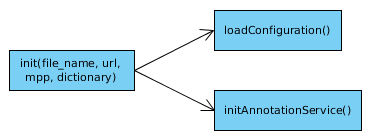
\includegraphics[scale=0.5]{img/ch_init.png}
		\caption{Call hierarchy of \texttt{init(file{\textunderscore}name, url, mpp)}}
		\label{figB_init}
	\end{center}
\end{figure}


\subsubsection{function initAnnotationService()}
\texttt{initAnnotationService()} selects the navigation tool (via \texttt{selectTool()}), creates the OSDV and its scalebar. It then opens the tile source at the URL specified in the \texttt{init(file{\textunderscore}path, url, mpp)} function. Additionally, event handlers to are set up to react to:
\begin{itemize}
	\item mouse interaction
	\item opening of a WSI
	\item zooming
\end{itemize}
Furthermore, the toolbar is initialized.

Once a tile source was opened, the AO is initialized (via \texttt{initAnnotationOverlay()}) and the saved annotations are requested (via \texttt{loadJson()}, see fig. \ref{figB_initAS}).

\begin{figure}[H]
	\begin{center}
		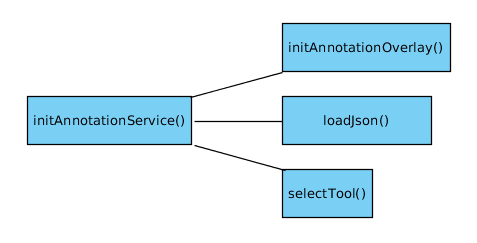
\includegraphics[scale=0.5]{img/ch_initAS.png}
		\caption{Call hierarchy of \texttt{initAnnotationService()}}
		\label{figB_initAS}
	\end{center}
\end{figure}


\subsubsection{function initAnnotationOverlay()}
\texttt{initAnnotationOverlay()} creates the ASV's AO. The AO is transformed to the size of the OSDV via the \texttt{transform()} function.


\subsection{Data management functions}

\subsubsection{function loadConfiguration()}
\texttt{loadConfiguration()} requests and parses the content of the configuration file from the ASS. Furthermore, it requests the list of available dictionaries (via \texttt{getDictionaryList()}) and loads the content of the dictionary specified in the configuration (via \texttt{loadDictionary(path)}, see fig. \ref{figB_loadConfig}).

\begin{figure}[H]
	\begin{center}
		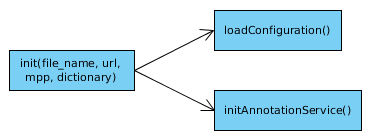
\includegraphics[scale=0.5]{img/ch_init.png}
		\caption{Call hierarchy of \texttt{loadConfiguration()}}
		\label{figB_loadConfig}
	\end{center}
\end{figure}


\subsubsection{function getDictionaryList()}
\texttt{getDictionaryList()} requests a list of all dictionaries from the ASS. The received list is then added as a clickable list to the toolbar.


\subsubsection{function loadDictionary(path)}
\emph{Parameters:\\
	path: file path of the requested dictionary\\ \\
}
\texttt{loadDictionary(path)} requests the content of the dictionary file at \emph{path} from the ASS. The response is either a list of entries, which are then added to the list of available labels in the toolbar (via \texttt{appendLabelsToList()}), or a -1, if no dictionary was found. In this case, the ASV forces the user to create a new, empty dictionary (via \texttt{createNewDictionary(isCancelable)}, see fig. \ref{figB_loadDict}).

\begin{figure}[H]
	\begin{center}
		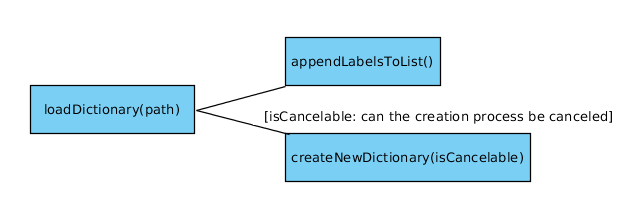
\includegraphics[scale=0.5]{img/ch_loadDict.png}
		\caption{Call hierarchy of \texttt{loadDictionary(path)}}
		\label{figB_loadDict}
	\end{center}
\end{figure}


\subsubsection{function loadJson()}
\texttt{loadJson()} requests the saved annotations for the provided WSI. If an annotation file could be loaded by the ASS, a list of region data is returned. Each entry of the region data list is then turned into an actual region and added to the region list (via \texttt{newRegion(arg, imageNumber)}, see fig. \ref{figB_loadJson}).

\begin{figure}[H]
	\begin{center}
		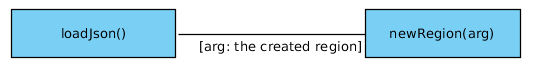
\includegraphics[scale=0.5]{img/ch_loadJson.png}
		\caption{Call hierarchy of \texttt{loadJson()}}
		\label{figB_loadJson}
	\end{center}
\end{figure}


\subsubsection{function createNewDictionary(isCancelable)}
\emph{Parameters:\\
	isCancelable: 1 if the process can be canceled without providing a valid dictionary name, 0 otherwise\\ \\
}
\texttt{createNewDictionary(isCancelable)} opens a prompt and asks the user to provide a name for the dictionary to create. If \emph{isCancelable} is true (1), the prompt can be closed and the creation process is canceled. If it is false (0), the prompt will be shown until a valid name was provided.

After creation of the new dictionary it is selected as active one (and its empty content is loaded via \texttt{loadDictionary(path)}) and the list of available dictionaries is updated (via \texttt{getDictionaryList()}, see fig. \ref{figB_createDict}).

\begin{figure}[H]
	\begin{center}
		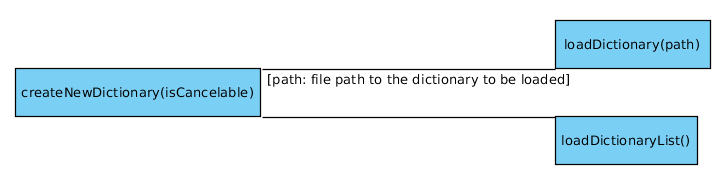
\includegraphics[scale=0.45]{img/ch_createDict.png}
		\caption{Call hierarchy of \texttt{createNewDictionary(isCancelable)}}
		\label{figB_createDict}
	\end{center}
\end{figure}


\subsection{GUI functions}

\subsubsection{function selectTool()}
\texttt{selectTool()} changes the mouse cursor to the icon of the currently selected tool.


\subsubsection{function transform()}
\texttt{transform()} resizes the AO to fit the view bounds of the OSDV.


\subsubsection{function appendLabelsToList()}
\texttt{appendLabelsToList()} first clears the currently shown list of labels. Then it iterates of the list of available labels (from the configuration) and creates a new, clickable label entry and adds it to the label list (via \texttt{appendLabelToList(label)}. Once all labels are created, the first entry is selected automatically (via \texttt{selectNextLabel()}, see fig. \ref{figB_appendLabels}).

\begin{figure}[H]
	\begin{center}
		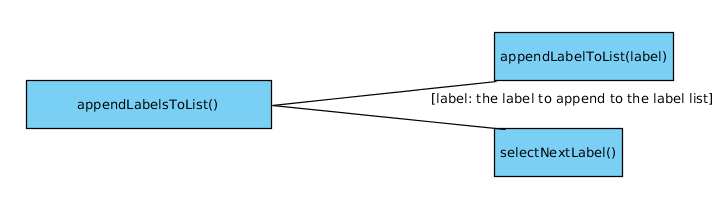
\includegraphics[scale=0.5]{img/ch_appendLabels.png}
		\caption{Call hierarchy of \texttt{appendLabelsToList()}}
		\label{figB_appendLabels}
	\end{center}
\end{figure}


\subsubsection{function appendLabelToList(label)}
\emph{Parameters:\\
	label: name of the new label
}
\texttt{appendLabelToList(label)} creates a new, clickable label for label list in the toolbar. It adds a click listener (via \texttt{singleClickOnLabel()}) to it and then selects it (via \texttt{selectLabel(el)}, see fig. \ref{figB_appendLabel}).

\begin{figure}[H]
	\begin{center}
		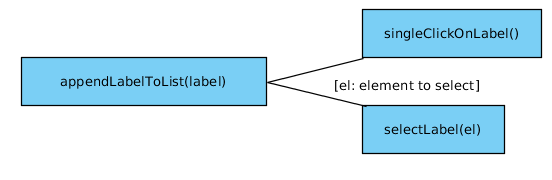
\includegraphics[scale=0.5]{img/ch_appendLabel.png}
		\caption{Call hierarchy of \texttt{appendLabelToList(label)}}
		\label{figB_appendLabel}
	\end{center}
\end{figure}


\subsubsection{function selectNextLabel()}
\texttt{selectNextLabel()} selects the next label in the toolbar list. If the currently selected label is the last one, the first entry is selected (via \texttt{selectLabel(el)}, see fig. \ref{figB_selectNextl}).

\begin{figure}[H]
	\begin{center}
		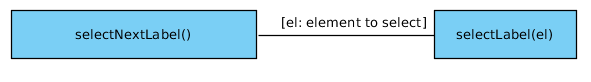
\includegraphics[scale=0.5]{img/ch_selectNext.png}
		\caption{Call hierarchy of \texttt{selectNextLabel(label)}}
		\label{figB_selectNextl}
	\end{center}
\end{figure}


\subsubsection{function selectLabel(el)}
\emph{Parameters:\\
	el: HTML element to select\\ \\
}
\texttt{selectLabel(el)} selects the provided element \emph{el} from the toolbar label list.


\subsubsection{function newLabel()}
\texttt{newLabel()} creates a new label for the toolbar's label list. The created label is also added to the dictionary and persisted there (via \texttt{saveDictionary()}). The function automatically generates a uid (via \texttt{uniqueID()}) and color (via \texttt{regionHashColor(label)}, see fig. \ref{figB_newLabel}).

\begin{figure}[H]
	\begin{center}
		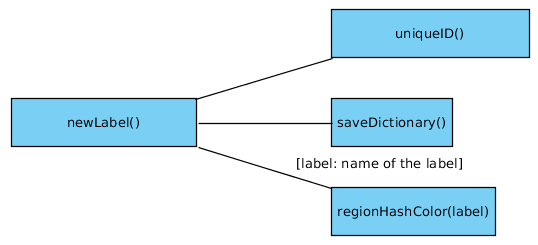
\includegraphics[scale=0.5]{img/ch_newLabel.png}
		\caption{Call hierarchy of \texttt{newLabel()}}
		\label{figB_newLabel}
	\end{center}
\end{figure}


\subsection{Region functions}
\subsubsection{function newRegion(arg)}
\emph{Parameters:\\
	arg: argument object (either a complete region or path and coordinate information)\\ \\
}
\texttt{newRegion(arg)} creates a new region from the information provided in \emph{arg} and adds it to the region list.


\subsubsection{function selectRegion(reg)}
\emph{Parameters:\\
	reg: region to select\\ \\
}
\texttt{selectRegion(reg)} selects the provided region.


\subsubsection{function deselectRegion(reg)}
\emph{Parameters:\\
	reg: region to deselect\\ \\
}
\texttt{deselectRegion(reg)} deselects the provided region.


\subsubsection{function findContextRegion(region1)}
\emph{Parameters:\\
	region1: region to find the context to\\ \\
}
\texttt{findContextRegion(region1)} finds the context of the provided region. The label of each region that crosses, touches, surrounds or is surrounded by \emph{region1} is considered as context. Too avoid data redundancy, each label will only be added once to the context of region1 (via \texttt{isRegionAlreadyReferenced(region1, region2)}, see fig. \ref{figB_findContext}).

\begin{figure}[H]
	\begin{center}
		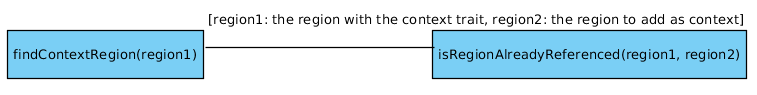
\includegraphics[scale=0.4]{img/ch_findContext.png}
		\caption{Call hierarchy of \texttt{findContextRegion()}}
		\label{figB_findContext}
	\end{center}
\end{figure}


\subsubsection{function isRegionAlreadyReferenced(region1, region2)}
\emph{Parameters:\\
	region1: region with the context to check\\
	region2: region whose label is checked for\\ \\
}
\texttt{isRegionAlreadyReferenced(region1, region2)} checks if region1's context already contains region2’s label.


\subsubsection{function removeRegion(reg)}
\emph{Parameter:\\
	reg: the region to remove\\ \\
}
\texttt{removeRegion(reg)} deletes the provided region.


\subsubsection{function findRegionByUID(uid)}
\emph{Parameter:\\
	uid: unique id of the region to find\\ \\
}
\texttt{findRegionByUID(uid)} finds a region with the provided id.


\subsubsection{function toggleRegions(uid)}
\emph{Parameters:\\
	uid: the label uid of the regions to toggle in their visibility\\ \\
}
\texttt{toggleRegions(uid)} turns all regions of the corresponding label (in-)visible. If one of the regions to be toggled is currently selected it is deselected (via \texttt{deselectRegion(reg)}, see fig. \ref{figB_toggleRegions}).

\begin{figure}[H]
	\begin{center}
		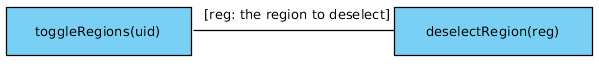
\includegraphics[scale=0.5]{img/ch_toggleRegions.png}
		\caption{Call hierarchy of \texttt{toggleRegions(uid)}}
		\label{figB_toggleRegions}
	\end{center}
\end{figure}


\subsubsection{function toggleAllRegions()}
\texttt{toggleAllRegions()} toggles the visibility of all regions.


\subsection{Interaction functions}
\subsubsection{function singleClickOnLabel(event)}
\emph{Parameters:\\
	event: the click event\\ \\
}
\texttt{singleClickOnLabel(event)} handles the click on a label in the toolbar's label list. Depending on what element inside the label is clicked, the following happens:
\begin{itemize}
	\item the visibility of all regions with the corresponding label is toggled on/off (via \texttt{toggleRegions(uid)})
	\item a window to open the annotation style (stroke width and color, alpha value, region color) is shown (via \texttt{changeRegionAnnotationStyle(uid)})
	\item the clicked label is selected (via \texttt{selectLabel(el)})
\end{itemize}

See fig. \ref{figB_singleClickLabel} for the call hierarchy of \texttt{singleClickOnLabel(event)}.

\begin{figure}[H]
	\begin{center}
		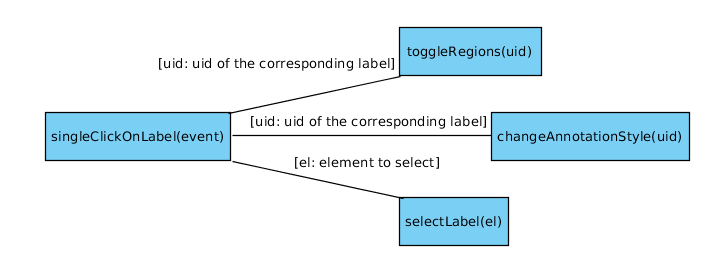
\includegraphics[scale=0.5]{img/ch_singleClickLabel.png}
		\caption{Call hierarchy of \texttt{singleClickOnLabel(event)}}
		\label{figB_singleClickLabel}
	\end{center}
\end{figure}


\subsubsection{function changeRegionAnnotationStyle(uid)}
\emph{Parameters:\\
	uid: the uid of the corresponding label\\ \\
}
\texttt{changeRegionAnnotationStyle(uid)} changes the annotation style (storke width and color, region color, region alpha value) for all regions corresponding to the label uid.


\subsubsection{function addPoi(event)}
\emph{Parameters:\\
	event: the click event\\ \\
}
\texttt{addPoi(event)} requests the server to run the segmentation script and provides it with the x and y coordinate the POI was placed at. Once the server returns with a valid answer (the image coordinates of the ROIs enclosing path), the coordinates are converted from image coordinates into AO coordinates (via \texttt{imgToPathCoordinates(point)}) and the ROI is enclosed by a path drawn along those AO coordinates. Then, a new region is created (via \texttt{newRegion(arg)}) and its checked for context (via \texttt{findContextRegion(region1)}).

If the ASS returns a "404 Not Found", an alert is shown and the currently selected POI tool is reset to the navigation tool (via \texttt{clearToolSelection()}).

Fig. \ref{fig_Bpoi} shows the call hierarchy of \texttt{addPoi(event)}.

\begin{figure}[H]
	\begin{center}
		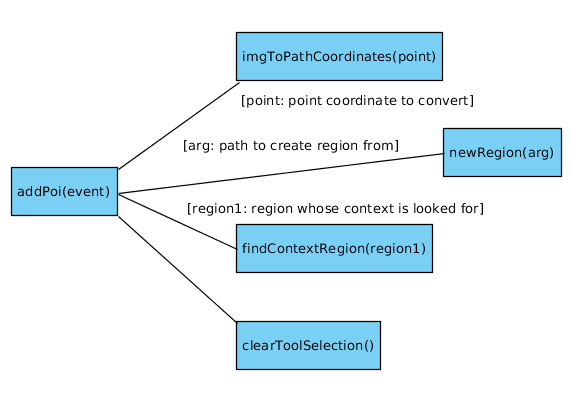
\includegraphics[scale=0.5]{img/ch_addPoi.png}
		\caption{Call hierarchy of \texttt{addPoi(event)}}
		\label{fig_Bpoi}
	\end{center}
\end{figure}


\subsection{Internal functions}

\subsubsection{UniqueID()}
\texttt{UniqueID()} creates a unique id and returns it.


\subsubsection{function regionHashColor(name)}
\emph{Parameters:\\
	name: name of a label\\ \\
}
\texttt{regionHashColor(name)} generates a color (rgba, with a = default alpha from configuration) from the hash value of the provided name.

\subsubsection{function convertPathToImgCoordinates(point)}
\emph{Parameters:\\
	point: point coordinate to convert\\ \\
}
\texttt{convertPathToImgCoordinates(point)} converts a point coordinate from the AO to a point coordinate in the OSDV's image.


\subsubsection{function convertImgToPathCoordinates(point)}
\emph{Parameters:\\
	point: point coordinate to convert\\ \\
}
\texttt{convertImgToPathCoordinates(point)} converts a point coordinate from the OSDV's image to a point coordinate in the AO.

\subsubsection{function mouseDown(x,y)}
\emph{Parameters:\\
	x: x coordinate of when left mouse button was pushed down\\
	y: y coordinate of when left mouse button was pushed down\\ \\
}
\texttt{mouseDown(x,y)} listens to mouse click events. It is called, once the mouse button is pushed down. The function handles every interaction the following interactions:
\begin{itemize}
	\item create region in free hand and polygon drawing mode (via \texttt{newRegion(arg)})
	\item add a new segment to a path in polygon drawing mode
	\item close a region's path in polygon mode, once a segment is clicked the second time (via \texttt{finishDrawingPolygon(closed)})
	\item select a clicked region (via \texttt{selectRegion(reg)})
\end{itemize}

See fig. \ref{figB_mouseDown} for the call hierarchy of \texttt{mouseDown(x,y)}.

\begin{figure}[H]
	\begin{center}
		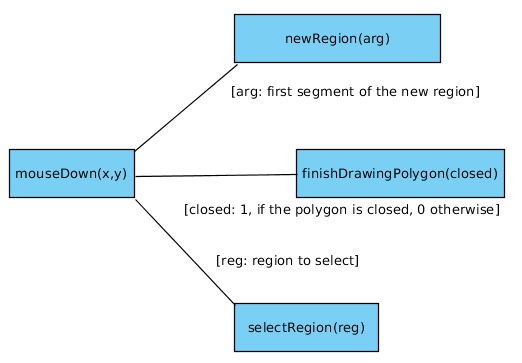
\includegraphics[scale=0.5]{img/ch_mouseDown.png}
		\caption{Call hierarchy of \texttt{mouseDown(x,y)}}
		\label{figB_mouseDown}
	\end{center}
\end{figure}


\subsubsection{function mouseDrag(x,y,dx,dy)}
\emph{Parameters:\\
	x: x coordinate with current mouse position\\
	y: y coordinate with current mouse position\\
	dx: delta of current and former mouse position in x \\
	dy: delta of current and former mouse position in y\\ \\
}
\texttt{mouseDrag(x,y,dx,dy)} handles all mouse interaction that happens with a pushed down left mouse button:
\begin{itemize}
	\item add new segment to path in free hand drawing mode (including conversion image coordinate $\rightarrow$ AO coordinate and AO coordinate $\rightarrow$ image coordinate\footnote{
		See subsection \ref{sec4_asvFrameworks} - Paper.js.
	}, see fig. \ref{figB_mouseDrag})
	\item move region
	\item move segment in region
\end{itemize}

\begin{figure}[H]
	\begin{center}
		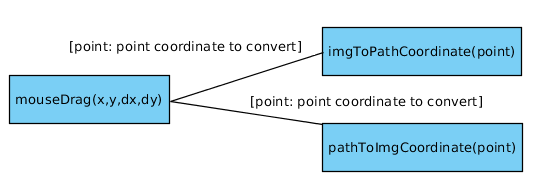
\includegraphics[scale=0.5]{img/ch_mouseDrag.png}
		\caption{Call hierarchy of \texttt{mouseDrag(x,y,dx,dy)}}
		\label{figB_mouseDrag}
	\end{center}
\end{figure}


\subsubsection{function mouseUp()}
When in free hand drawing mode, the \texttt{mouseUp()} function closes a region's path, once the left mouse button is released (including conversion as in the first item of \texttt{mouseDrag(x,y,dx,dy})).

When in distance measurement mode, the distance tooltip is removed upon release of the left mouse button.


\subsubsection{function finishDrawingPolygon(closed)}
\emph{Parameters:\\
	closed: 1 if path should be closed, 0 otherwise\\ \\
}
\texttt{finishDrawingPolygon(closed)} finishes the drawing process of a region's path in polygon drawing mode. If closed is true (1), the first and last segment will be connected.


\subsubsection{function getDistance()}
\texttt{getDistance()} calculates the euclidian distance $d$ between pixels $p_a$ and $p_b$ (see eq. \ref{eq:distance}\cite{Strang03}) of a special path called \emph{ruler} that is exclusively used for the distance measurement tool.
\begin{equation}\label{eq:distance}
	d = \sqrt{
	 	(p_b.x - p_a.x)^2 + (p_b.y - p_a.y)^2
	}
\end{equation}

%-----------------------------------------------------------------------



\subsubsection{function annotationStyle(label)}
\subsubsection{function setRegionColor()}


\subsubsection{function cmdDeleteSelected()}
\subsubsection{function clearToolSelection()}

\subsubsection{function saveJson(json, filePath)}
\subsubsection{function saveConfig()}
\subsubsection{function saveDictionary()}
\subsubsection{function saveRegions()}

\subsubsection{function resizeAnnotationOverlay()}

\subsubsection{function toggleDictPicker()}
\subsubsection{function dictListClick(index)}

\subsubsection{function help(show)}
\subsubsection{function toggleMenu ()}

\subsubsection{\$(document).keydown(function(e)}
\subsubsection{function selectToolOnKeyPress(id)}
\subsubsection{\$(document).keyup(function(e)}

	\chapter{Tessellation Service Documentation}
\label{secC}
The TS is openly available at GitHub and comes with instructions for usage and installation. The Repository can be found at:

\url{https://github.com/SasNaw/TessellationService}

%Once \texttt{save{\textunderscore}image(image, region, slide{\textunderscore}name, *tiles)} is called, the destination for the output is set, either to a location provided via -o or in the same directory as the TS. If the provided directory should not exist, it will be created. To keep correspondence to the label of the ROI, The provided image is saved in a directory with the name of the (see line 2 - 7).  

% # L = R * 299/1000 + G * 587/1000 + B * 114/1000

and the annotated regions extracted from the corresponding JSON file. After the arguments and parameters are parsed, the script's \texttt{run()} method is called, which starts the extraction process for all input elements:


\begin{lstlisting}[frame=single, language=python, title=\texttt{run()} from TessellationService.py]
def run(input):
for element in input:
# input is folder:
if(os.path.isdir(element)):
files_from_dir(element)
# input is file:
elif(os.path.isfile(element)):
regions_from_file(element)
\end{lstlisting}





As stated in section \ref{sec5_method}, each input element can be a file or a dictionary. Therefore, the individual entries must be examined. If the current element is a WSI or DZI, the extraction begins right away (see line 8). If it is a directory, \texttt{files{\textunderscore}from{\textunderscore}dir(dir)} will be called (see line 5) and search for valid files, including all contained subdirectories:

\begin{lstlisting}[frame=single, language=python, title=\texttt{files{\textunderscore}from{\textunderscore}dir(dir)} from TessellationService.py]
def files_from_dir(dir):
if not dir.endswith('/'):
dir = dir + '/'
contents = os.listdir(dir)
for content in contents:
if os.path.isdir(dir + content):
if not content.endswith('_files'):
files_from_dir(dir + content)
else:
regions_from_file(dir + content)
\end{lstlisting}

After the contents of the directory are received (see line 4), they are evaluated further (see line 5 - 10). If the input directory contains subdirectories, \texttt{files{\textunderscore}from{\textunderscore}dir(dir)} is called recursively for each one of them, until the end of each directory tree is reached (see line6 - 8 in \texttt{files{\textunderscore}from{\textunderscore}dir(dir)}). Otherwise, the extraction process is started for the detected file (see line 9 - 10 in \texttt{files{\textunderscore}from{\textunderscore}dir(dir)}). Directories ending in \emph{"{\textunderscore}files"} are excluded since they only contain the tiled images for an associated DZI metadata file and a metadata.txt, if they were converted by the CS\footnote{
	Compare chapter \ref{sec3_cs}
} (see line 7 in \texttt{files{\textunderscore}from{\textunderscore}dir(dir)}).
\end{appendices}

\bibliographystyle{plain}

\bibliography{./bibl/bibl}
\listoffigures
\listoftables
%TODO deine Nomenklatur hat grade sowohl Neural Network als auch Neural Networks als NN ausgezeichnet (siehe letzte seite des pdfs).
\printnomenclature

\end{document}
